\documentclass{article}

\def\ParSkip{} 
\input{../../common/ryantibs}
\usepackage[normalem]{ulem}

\title{Conformal Prediction \\ \smallskip
\large Advanced Topics in Statistical Learning, Spring 2024 \\ \smallskip
Ryan Tibshirani }
\date{}

\begin{document}
\maketitle
\RaggedRight
\vspace{-50pt}

\section{Introduction}

Conformal prediction is a relatively new framework for quantifying uncertainty
in the predictions made by arbitrary prediction algorithms. Fundamentally, it
does so by converting an algorithm's predictions into prediction sets, which
have strong finite-sample coverage properties. 

The idea behind conformal prediction was born out of conversations between
Vladimir Vovk and his colleagues, including Alexander Gammerman and Vladimir
Vapnik (who was visiting the university), in the mid 1990s at Royal Holloway,
University of College London. The definitive reference is
\citet{vovk2005algorithmic}. This remained a topic of intense interest for Vovk
and collaborators for many years, up through current day. It is Larry Wasserman
who brought about the interest in the statistics community, and inspired
Carnegie Mellon University colleagues including Jing Lei (and the author of
these lecture notes), to collaborate on conformal prediction in the mid
2010s. This lecture will draw mostly from the language for conformal prediction
developed in \citet{lei2018distribution, tibshirani2019conformal}.    

The community working on conformal prediction remained fairly small for most of
its short history, until fairly recently---just the last few years,
really---when it exploded in popularity in the machine learning community. As
such, there will be a lot of interesting work about conformal prediction that
we will not be covering. A nice recent overview is
\citet{angelopoulos2023gentle}. The last section of that monograph provides some 
sense of the current trends in the field.      

\subsection{A lofty goal?}

\def\hC{\hat{C}}
\def\hq{\hat{q}}
\def\Quantile{\mathrm{Quantile}}

The basic goal of conformal prediction is as follows. Let $(X_i,Y_i) \sim P$,
$i=1,\dots,n$ be i.i.d.\ feature and response pairs, from a distribution 
$P$ on $\cX \times \cY$. For concreteness, we can think of the feature space as
say, $\cX = \R^d$, and the response space as $\cY = \R$, though this need not be 
the case in general. Let $\alpha \in (0,1)$ be and a nominal error level. Then
we want to find a \emph{prediction band}, 
\[
\hC_n : \cX \to \{ \text{subsets of $\cY$} \},
\]
with the property that for a new i.i.d.\ pair $(X_{n+1},Y_{n+1}) \sim P$,
\begin{equation}
\label{eq:coverage_goal}
\P\big( Y_{n+1} \in \hC_n(X_{n+1}) \big) \geq 1-\alpha,
\end{equation}
where the probability is over all of our data $(X_i,Y_i)$, $i=1,\dots,n+1$. 

On the one hand, without placing any assumptions on $P$, and without appealing
to asymptotics of any kind, this might seem like a really hard goal in
general. On the other hand, we can do something trivial to obtain it: for example,   
\[
\hC_n(X_{n+1}) = 
\begin{cases}
\cY & \text{with probability $1-\alpha$} \\
\emptyset & \text{with probability $\alpha$}
\end{cases}
\]
will always have exactly $1-\alpha$ coverage, that is, it will achieve
\eqref{eq:coverage_goal} with an equality.   

So the real question is this (albeit still somewhat vaguely-phrased): can we
achieve \eqref{eq:coverage_goal}, in finite samples, without any assumptions on
$P$, by doing something ``nontrivial''? In particular, we would like our
strategy to adapt to the hardness of the problem, in the following sense: the
more easily we can predict $Y_{n+1}$ from $X_{n+1}$, the smaller we would like
our set \smash{$\hC_n(X_{n+1})$} to be. 

\subsection{This is achieveable!}
\label{sec:no_features}

Perhaps remarkably, this last goal is actually achieveable, in a very general
way. As we will see in the coming sections, we can start with any algorithm that
produces a ``point predictor'' \smash{$\hf_n$} that predicts $Y_{n+1}$ from
$X_{n+1}$, and turn this into a ``set predictor'' \smash{$\hC_n$} that satisfies
\eqref{eq:coverage_goal}. 

The basic idea behind conformal prediction is two-fold. The first key idea can
actually be explained in a simpler context, \emph{where there are no features at
  all}, and we just have a sequence $Y_i \in \R$, $i=1,\dots,n$ of real-valued
response values. Suppose our goal is to find a one-sided prediction interval
\smash{$\hC_n = (-\infty, \hq_n]$} with
\begin{equation}
\label{eq:coverage_goal_y}
\P\big( Y_{n+1} \leq \hq_n \big) \geq 1-\alpha.
\end{equation}
Given this goal \eqref{eq:coverage_goal_y}, a natural place to start would be to
set \smash{$\hq_n$} to be the level $(1-\alpha)$ sample quantile of
$Y_1,\dots,Y_n$, which we denote by  
\[
\hq_n = \Quantile\bigg( 1-\alpha; \, \frac{1}{n} \sum_{i=1}^n \delta_{Y_i}
\bigg), 
\]
with $\delta_a$ denoting a point mass at $a$, and hence \smash{$\frac{1}{n}
  \sum_{i=1}^n \delta_{Y_i}$} denoting the empirical distribution of
$Y_1,\dots,Y_n$. But this would only give use the approximate result 
\[
\P(Y_{n+1} \leq \hq_n) \approx 1-\alpha.
\]
This becomes exact as $n \to \infty$, under standard conditions (that ensure
convergence of the sample quantile to the population quantile). So can we
instead get something that satisfies \eqref{eq:coverage_goal_y} in
finite-sample?     

\paragraph{First key idea: use ranks to form adjusted quantiles.} 

This is where the first key idea behind conformal prediction comes in (which in
a sense traces back to work on rank-based statistics and permutations by Fisher
and Pitman in the 1930s). As $Y_{n+1}$ is i.i.d.\ with $Y_1,\dots,Y_n$, then  
\begin{equation}
\label{eq:rank_uniform_y}
\text{the rank of $Y_{n+1}$ is uniformly distributed over the values 
  $Y_1,\dots,Y_{n+1}$}.
\end{equation}
This means that 
\begin{equation}
\label{eq:compare_y1}
\P\Big( \text{$Y_{n+1} \leq $ the $\lceil (1-\alpha)(n+1) \rceil$ smallest of
  $Y_1,\dots,Y_{n+1}$} \Big) \geq 1-\alpha,  
\end{equation}
which is in turn equivalent to\footnote{To see this, consider the complement of
  the events (inside the probabilities) in \eqref{eq:compare_y1},
  \eqref{eq:compare_y2}. Abbreviate \smash{$k = \lceil (1-\alpha)(n+1)
    \rceil$}. Then $Y_{n+1} >$ the $k$ smallest of $Y_1,\dots,Y_{n+1}$ is
  clearly an equivalent statement to $Y_{n+1} >$ the $k$ smallest of
  $Y_1,\dots,Y_n$, since $Y_{n+1}$ can never be strictly larger than
  itself. That said, this argument really only makes sense for $k \leq n$, and
  for $k = n+1$, which occurs if $\alpha < 1/(n+1)$, then \smash{$\lceil
    (1-\alpha)(n+1) \rceil = n+1$}, then we have to interpret the $(n+1)$
  smallest of $Y_1,\dots,Y_n$ as being $+\infty$ to equate
  \eqref{eq:compare_y1}, \eqref{eq:compare_y2}. This is the consistent with
  interpreting the quantile function in \eqref{eq:quantile_y2} to return
  $+\infty$ when the input level is $\geq 1$.}          
\begin{equation}
\label{eq:compare_y2}
\P\Big( \text{$Y_{n+1}\leq $ the $\lceil (1-\alpha)(n+1) \rceil$ smallest of
  $Y_1,\dots,Y_n$} \Big) \geq 1-\alpha. 
\end{equation}
The last step is critical: note that we have moved from a comparison between 
$Y_{n+1}$ and a an order statistic of $Y_1,\dots,Y_{n+1}$ in
\eqref{eq:compare_y1} to a comparison between $Y_{n+1}$ and an order statistic
of $Y_1,\dots,Y_n$ in \eqref{eq:compare_y2}. This is key, because what is on the
right-hand side of the $\leq$ sign in \eqref{eq:compare_y2} is \emph{computable
  from just the first $n$ points}. Accordingly, by defining  
\begin{equation}
\label{eq:quantile_y1}
\text{$\hq_n = \lceil (1-\alpha)(n+1) \rceil$ smallest of $Y_1,\dots,Y_n$}, 
\end{equation}
we have precisely achieved \eqref{eq:coverage_goal_y}. 

The formulation in \eqref{eq:quantile_y1} is arguably the most intuitive way to
remember how to achieve coverage. There are other equivalent formulations. One
such equivalent formulation (we will see more later on) is
\begin{equation}
\label{eq:quantile_y2}
\hq_n = \Quantile\bigg( \frac{\lceil (1-\alpha)(n+1) \rceil}{n}; \,
\frac{1}{n} \sum_{i=1}^n \delta_{Y_i} \bigg).
\end{equation}
In this way, we can also see the solution here as simply to taking the sample 
quantile at an adjusted level: we use \smash{$\lceil (1-\alpha)(n+1) \rceil /
  n$}, instead of $1-\alpha$, which is a sort of finite-sample correction. But
in our opinion, the fact that  \eqref{eq:quantile_y2} achieves the coverage
guarantee is less obvious; only through its equivalence to
\eqref{eq:quantile_y1}---and then the equivalence to the precedings displays in
\eqref{eq:compare_y2}, \eqref{eq:compare_y1}, \eqref{eq:rank_uniform_y}---does
this become transparent. A very simple illustration of the key idea here is
given in Figure \ref{fig:illustration}.     

\begin{figure}[htb]
\centering
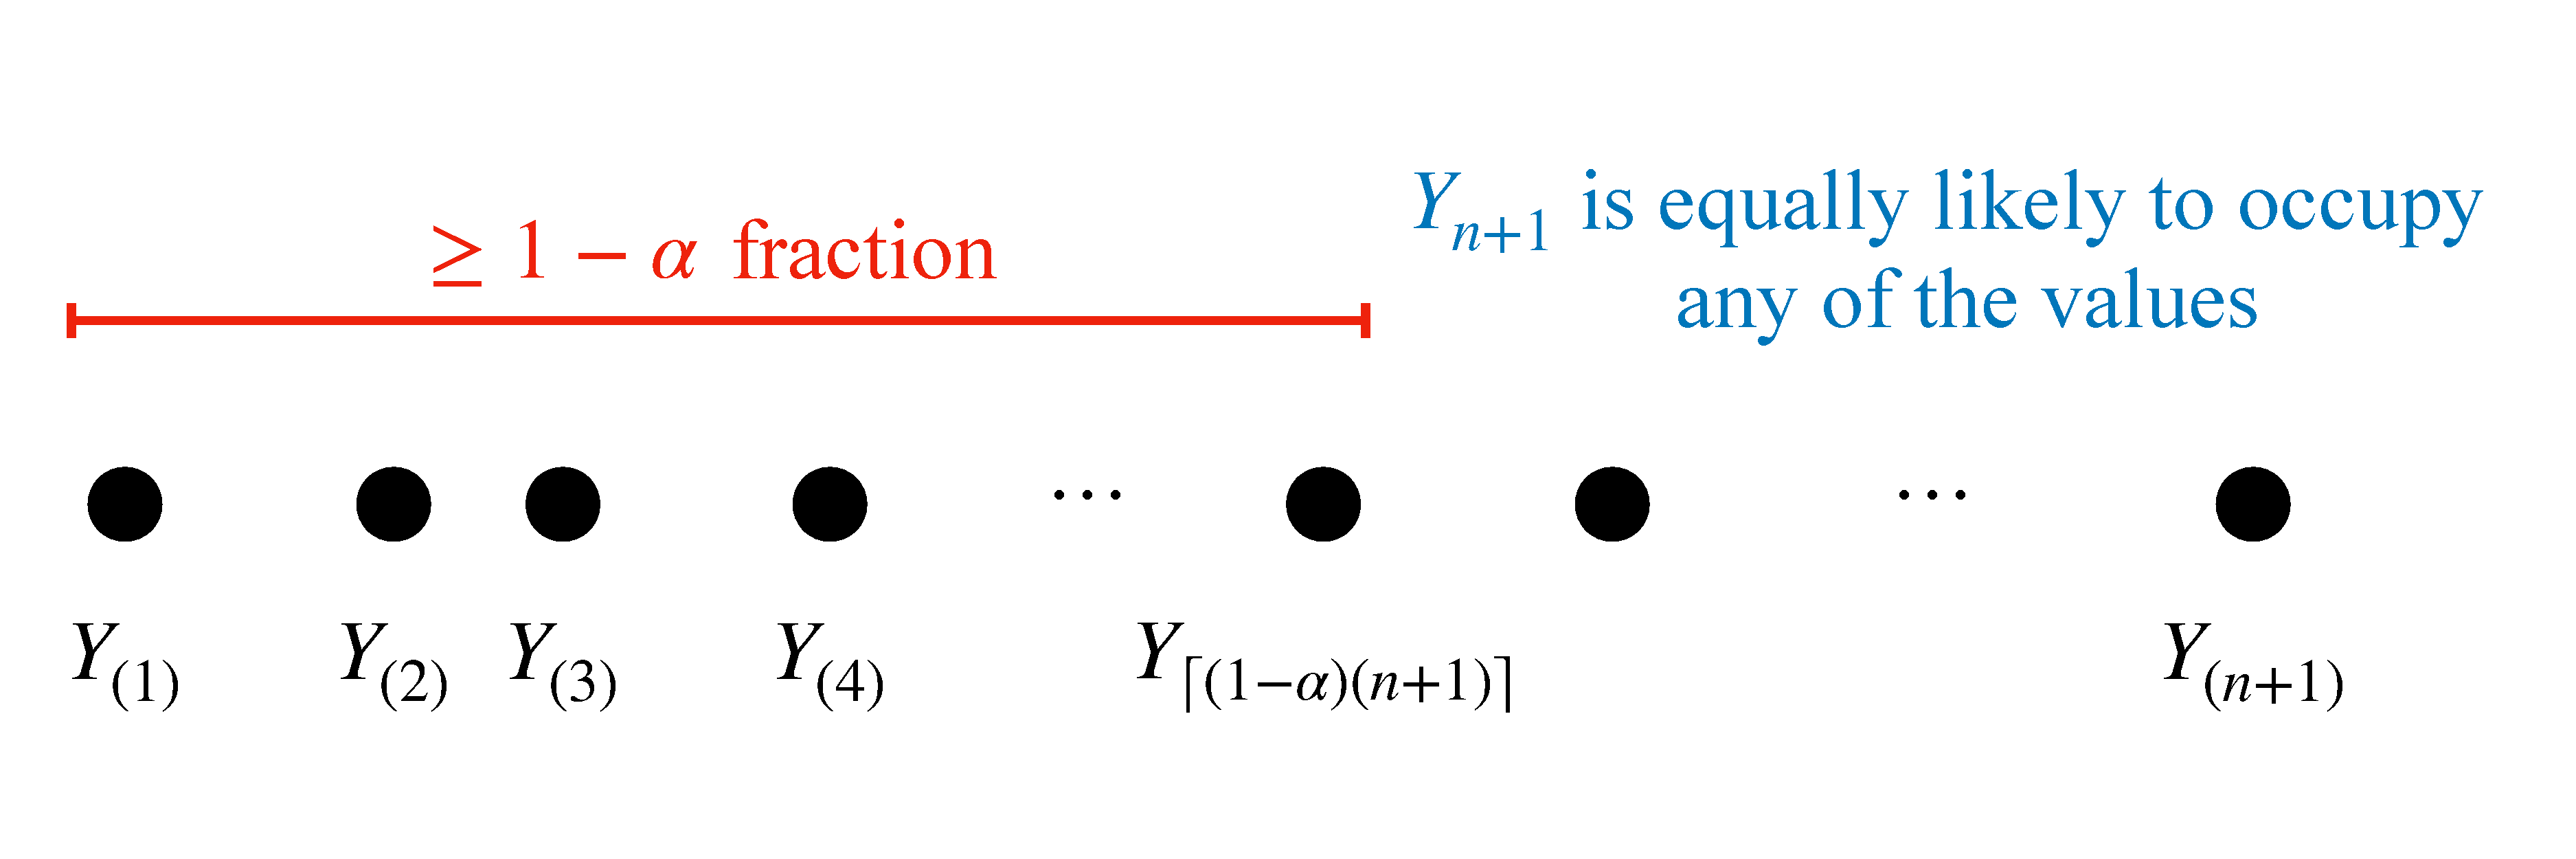
\includegraphics[width=0.7\textwidth]{illustration.pdf}
\caption{\it Illustration of the first key idea in conformal prediction, as
  stated in \eqref{eq:rank_uniform_y}, \eqref{eq:compare_y1}. Note also that we
  have the sharpened version \eqref{eq:compare_y3} when there are almost surely
  no ties.}    
\label{fig:illustration}
\end{figure}

\paragraph{\sout{Love} Exchangeability is all you need.}

\def\deq{\overset{d}{=}}

Looking back at \eqref{eq:rank_uniform_y}, all that we need for this to hold is 
that $Y_1,\dots,Y_{n+1}$ are \emph{exchangeable}, which is a weaker than the  
i.i.d.\ assumption. Recall that exchangeability of $Y_1,\dots,Y_{n+1}$ means
that their joint distribution is unchanged under permutations:
\[
(Y_1, \dots, Y_{n+1}) \deq (Y_{\sigma(1)} ,\dots, Y_{\sigma(n+1)}), \quad
\text{for all permutations $\sigma$}.
\]

\paragraph{Coverage upper bound when there are no ties.}

If there are almost surely no ties between $Y_1,\dots,Y_{n+1}$ (or we use a
suitably random tie-breaking rule) then the statement in \eqref{eq:compare_y1}
can be sharpened to an equality,  
\begin{equation}
\label{eq:compare_y3}
\P\Big( \text{$Y_{n+1} \leq$ the $\lceil (1-\alpha)(n+1) \rceil$ smallest of
  $Y_1,\dots,Y_{n+1}$} \Big) = \frac{\lceil (1-\alpha)(n+1) \rceil}{n+1}. 
\end{equation}
Simply upper bounding the right-hand side above gives
\begin{equation}
\label{eq:compare_y4}
\P\Big( \text{$Y_{n+1} \leq$ the $\lceil (1-\alpha)(n+1) \rceil$ smallest of
  $Y_1,\dots,Y_{n+1}$} \Big) < (1-\alpha) + \frac{1}{n+1}. 
\end{equation}
Carrying on from by the same logic as before leads to the sharpened conclusion, 
\begin{equation}
\label{eq:coverage_twosided}
\P\big( Y_{n+1} \leq \hq_n \big) \in \Big[ 1-\alpha, \, 1-\alpha + \frac{1}{n+1}
\Big).  
\end{equation}
with \smash{$\hq_n$} still defined as in \eqref{eq:quantile_y1}. To be clear,
the lower bound on coverage in \eqref{eq:coverage_twosided} always holds, and
the upper bound holds under the assumption that there are almost surely no ties.  

\paragraph{Naive attempt to lift this idea to regression problems.} 

Now let's try to lift the first key idea to a regression setting, where we
observe both $X_i \in \cX$ and $Y_i \in \R$, $i=1,\dots,n$, and want a
prediction set for $Y_{n+1}$ based on $X_{n+1}$. Suppose that \smash{$\hf_n$} is  
any point predictor, trained on $(X_i,Y_i)$, $i=1,\dots,n$, such that (to put it 
informally)  
\[
\text{$\hf_n(x)$ predicts the value of $y$ that we expect to see at $x$.}  
\]
Then we could proceed naively as follows. We define (absolute) residuals made on 
the training set,     
\[
R_i = |Y_i - \hf_n(X_i)|, \quad i=1,\dots,n,
\]
and just as in \eqref{eq:quantile_y1}, let \smash{$\hq_n = \lceil
  (1-\alpha)(n+1) \rceil$ smallest of $R_1,\dots,R_n$}. We could then define
the prediction set to be \smash{$\hC_n(x) = \{ y : |y - \hf_n(x)| \leq \hq_n
  \}$}, or in other words
\[
\hC_n(x) = \big[ \hf_n(x) - \hq_n, \, \hf_n(x) + \hq_n \big], 
\]
in the hope that \smash{$Y_{n+1} \in \hC_n(X_{n+1})$} with probability at least
$1-\alpha$. However, 
\[
Y_{n+1} \in \hC_n(X_{n+1}) 
\iff R_{n+1} \leq \hq_n 
\iff \text{$R_{n+1} \leq \lceil (1-\alpha)(n+1) \rceil$ smallest of
  $R_1,\dots,R_n$},   
\]
and the latter event does \emph{not} hold with probability $1-\alpha$, because
\smash{$R_{n+1} = |Y_{n+1} - \hf_n(X_{n+1})|$} is \emph{not} exchangeable with 
$R_1,\dots,R_n$. 

The problem is that \smash{$\hf_n$} has already "seen" $(X_i,Y_i)$,
$i=1,\dots,n$ (since it was trained on them), but it has not yet seen
$(X_{n+1},Y_{n+1})$. Accordingly, the test residual $R_{n+1}$ will be generally
stochastically larger than the training residuals $R_1,\dots,R_n$, and so the
naive prediction set defined above will generally undercover. 

\section{Split conformal prediction}

Enter the second key idea behind conformal prediction, and \emph{split conformal
  prediction}, which is the simplest and most computationally efficient way to
carry out this idea. Split conformal prediction is the focus of this section,
and we stick to regression where responses are real-valued, so $\cY = \R$.  
The next section describes a (much more complicated) method that avoids
splitting the data. At the end of this lecture, we will consider classification,
where $\cY$ is discrete.     

\paragraph{Second key idea: construct scores symmetrically.}

In a nutshell, the second key idea in conformal prediction is to build residuals
in way that treats all of the data (that goes into determining their
distribution), including the test data, in a \emph{symmetric} fashion. This will
ensure that the residuals obey the exchangeability condition we require in order
to get coverage. 

Concretely, in split conformal prediction (split CP) we do the following. We
first divide the training set into two sets:   
\begin{itemize}
\item $D_1$, called the \emph{proper training set}; and
\item $D_2$, called the \emph{calibration set}.
\end{itemize}
We can think of these as sets of indices, so that $D_1,D_2$ are such that $D_1 
\cap D_2 = \emptyset$ and $D_1 \cup D_2 = \{1,\dots,n\}$. Let $n_1 = |D_1|$ and
$n_2 = |D_2|$. The next step is to fit our point predictor on proper training
points $(X_i,Y_i)$, $i \in D_1$, call it \smash{$\hf_{n_1}$}. Then we define 
calibration set residuals  
\[
R_i = |Y_i - \hf_{n_1}(X_i)|, \quad i \in D_2,
\]
a conformal quantile
\[
\text{$\hq_{n_2} = \lceil (1-\alpha)(n_2+1) \rceil$ smallest of $R_i$, $i \in
  D_2$},
\]
and a conformal set
\begin{equation}
\label{eq:cset_split}
\hC_n(x) = \big[ \hf_{n_1}(x) - \hq_{n_2}, \, \hf_{n_1}(x) + \hq_{n_2} \big],  
\end{equation}
The main guarantee we can get is that 
\begin{equation}
\label{eq:coverage_split}
\P\Big( Y_{n+1} \in \hC_n(X_{n+1}) \, \Big| \, (X_i,Y_i), \, i \in D_1 \Big) \in 
\Big[ 1-\alpha, \, 1-\alpha + \frac{1}{n_2+1} \Big),  
\end{equation}
where the lower bound on coverage always holds, and the upper bound holds under
the assumption that the residuals are almost surely distinct. Why? If we
condition on the proper training set $(X_i,Y_i)$, $i \in D_1$, then \emph{the
  calibration residuals $R_i$, $i \in D_2$ and the test residual \smash{$R_{n+1}
    = |Y_{n+1} - \hf_{n_1}(X_{n+1})|$} are all i.i.d.}, and therefore  
\[
Y_{n+1} \in \hC_n(X_{n+1}) 
\iff R_{n+1} \leq \hq_{n_2}  
\iff \text{$R_{n+1} \leq \lceil (1-\alpha)(n_2+1) \rceil$ smallest of $R_i$, $i 
  \in D_2$}  
\]
occurs (by our previous arguments) with probability at least $1-\alpha$, and at
most $1-\alpha+1/(n_2+1)$ if the residuals are almost surely distinct. 

\paragraph{Any score function will work.}

Above, we used absolute residuals as a negatively-oriented score function
(negatively-oriented meaning that lower values are better). But really, any
negatively-oriented score function will do, and the argument goes through
just as before. That is, suppose \smash{$V(x,y) = V((x,y); \hf_{n_1})$} assigns
a conformity score to the point $(x,y)$ based on \smash{$\hf_{n_1}$} (for
simplicity, we will generally drop the notational dependence on
\smash{$\hf_{n_1}$}). Define, generalizing the construction leading up to
\eqref{eq:cset_split}, calibration set scores
\[
R_i = V(X_i,Y_i), \quad i \in D_2, 
\]
and a conformal set
\[
\hC_n(x) = \Big\{ y : \text{$V(x,y) \leq \lceil (1-\alpha)(n_2+1) \rceil$
  smallest of $R_i$, $i \in D_2$} \Big\}. 
\]
Then we get the exact same guarantee as in \eqref{eq:coverage_split}, since
$R_i$, $i \in D_2$ and \smash{$R_{n+1} = V(X_{n+1},Y_{n+1})$} are all still
i.i.d., conditional on \smash{$\hf_{n_1})$}. This will be important later, as
we'll see how to move beyond the residual score to obtain better local
adaptivity in our prediction bands.        

Positively-oriented scores will work too, we can just negate them (to
make the negatively-oriented) before passing them through this
construction. This would result in a conformal set of the form
\[
\hC_n(x) = \Big\{ y : \text{$V(x,y) \geq \lfloor \alpha (n_2+1) \rfloor$
  smallest of $R_i$, $i \in D_2$} \Big\}.  
\]
An example of a naturally occurring positively-oriented scores will arise in the   
classification setting.

\paragraph{Quantile and CDF formulations.}

Keeping the conformity score generic (and negatively-oriented) for now, we note
that there are multiple equivalent formulations for the split conformal
prediction set:  
\begin{align}
\label{eq:cset_orig_split}
\hC_n(x) 
&= \Big\{ y : \text{$V(x,y) \leq \lceil (1-\alpha)(n_2+1) \rceil$ smallest of
  $R_i$, $i \in D_2$} \Big\} \\  
\label{eq:cset_quant_split}
&= \bigg\{ y : V(x,y) \leq \Quantile\bigg( \frac{\lceil (1-\alpha)(n_2+1)
  \rceil}{n_2}; \, \frac{1}{n_2} \sum_{i \in D_2} \delta_{R_i} \bigg) \bigg\} \\
\label{eq:cset_cdf_split}
&= \bigg\{ y : \frac{1}{n_2} \sum_{i \in D_2} 1\{ R_i \leq V(x,y) \} \leq
  \frac{\lceil (1-\alpha)(n_2+1) \rceil}{n_2} \bigg\}.   
\end{align}
The original formulation in \eqref{eq:cset_orig_split} is (we think) the most
intuitive. 

The second formulation in \eqref{eq:cset_quant_split} is of the form ``test
score $\leq$ adjusted quantile''. This form will be useful for generalizing
conformal prediction to use weights, which we will cover in the next lecture,
when we consider certain settings where the scores are no longer exchangeable. 

The third formulation \eqref{eq:cset_cdf_split} is expressed in terms of the
empirical cumulative distribution function (CDF) of $R_i$, $i \in D_2$. It is of 
the form ``CDF evaluated at test score $\leq$ adjusted level''. This is a useful
form when considering auxiliary randomization schemes, covered next. 

\paragraph{Auxiliary randomization to get exact coverage.*}  

It is worth noting that we can always use auxiliary randomization to get exact
coverage in our prediction sets, that is, to achieve $1-\alpha$ coverage in
\eqref{eq:coverage_split}. You can skip this without interrupting the flow of
understanding the ideas in the rest of this lecture, hence the asterisk. First,
rewrite the conformal set in its CDF form \eqref{eq:cset_cdf_split} as   
\[
\hC_n(x) = \bigg\{ y : \frac{1}{n_2+1} \sum_{i \in D_2} 1\{ R_i \leq V(x,y) \}
+ \frac{1}{n_2+1} \leq \frac{\lceil (1-\alpha)(n_2+1) \rceil}{n_2+1} \bigg\}.    
\]
This now compares the empirical CDF on the $n_2+1$ points: $R_i$, $i \in D_2$
and $V(x,y)$, to an adjusted level. To explain the auxiliary randomization 
mechanism, it helps to look at what happens at the (unknown) test point 
$(X_{n+1},Y_{n+1})$: let $R_{n+1} = V(X_{n+1},Y_{n+1})$ denote its score, and
let \smash{$\hat{F}_{n_2+1}$} denote the CDF of $R_i$, $i \in D_2$ and
$R_{n+1}$. Then   
\[
Y_{n+1} \in \hC_n(X_{n+1}) \iff \hat{F}_{n_2+1}(R_{n+1}) \leq \frac{\lceil 
  (1-\alpha)(n_2+1) \rceil}{n_2+1}, 
\]
which we know occurs with probability at least $1-\alpha$.

In general, if $Z$ has CDF $F$, then $F(Z)$ is always sub-uniform, meaning 
$\P( F(Z) \leq t) \leq t$ for any $t \in [0,1]$. This is another way of seeing
the coverage result stated above. Meanwhile, if $F$ is continuous, then $F(Z)$
will be precisely uniform, $\P( F(Z) \leq t) \leq t$ for any $t \in
[0,1]$. Furthermore, we can always take any CDF and make it continuous by
injecting auxiliary randomness, defining for $U \sim \mathrm{Unif}(0,1)$,
\[
F^*(z) = \lim_{y \to z^-} F(y) + U \cdot \Big( F(z) - \lim_{y \to z^-} F(y)
\Big).
\]

Returning to our conformal setting, we see that if we define a randomized
conformal prediction set based on auxiliary randomization of the empirical CDF, 
such that  
\[
Y_{n+1} \in \hC_n^*(X_{n+1}) \iff \hat{F}_{n_2+1}^*(R_{n+1}) \leq 1-\alpha,
\] 
then we will get coverage with probability exactly $1-\alpha$. Spelling it out
in more detail, this is the same as defining the randomized conformal set 
\[
\hC_n^*(x) = \bigg\{ y : \frac{1}{n_2+1} \sum_{i \in D_2} 1\{ R_i < V(x,y) \} 
+ \frac{U}{n_2+1} \bigg( \sum_{i \in D_2} 1\{ R_i = V(x,y) \} + 1 \bigg)
\leq 1-\alpha \bigg\},
\]
where $U \sim \mathrm{Unif}(0,1)$ is independent of everything else. To record
its guarantee, this set always satisfies  
\[
\P\Big( Y_{n+1} \in \hC_n^*(X_{n+1}) \, \Big| \, (X_i,Y_i), \, i \in D_1 \Big) = 
1-\alpha. 
\]

\subsection{Remarks}

Here we make some brief remarks about split conformal prediction. First, recall
that the naive prediction band---as covered at the end of Section
\ref{sec:no_features}---is generally going to undercover, drastically so when
\smash{$\hf_n$} overfits the training data. In a sense, we can think of the 
split conformal band \eqref{eq:cset_split} as being \emph{protected against
  overfitting}, since it based on comparing a test score to calibration set
scores, and in the overfitting regime, these will all be equally large (in
distribution).   

Second, note that the split conformal band \eqref{eq:cset_split} constructed
using absolute residual scores has width that is \emph{exactly constant in
  $x$}. This is not generally a good thing: it means that the band does not
adapt to the local hardness of the problem (how hard it is to predict at any
given $x$), as we will clearly see in an example to follow. However, this can be
addressed by changing the conformity score, as we will do in Section
\ref{sec:local_adaptivity}.    

Third and last, we note the following key fact: \emph{the better the point
  predictor \smash{$\hf_{n_1}$}} (from the proper training set), \emph{the
  tighter the prediction band will be}. Both experiments and theory corroborate
this claim; see, e.g., \citet{lei2018distribution}, and Figure
\ref{fig:experiments}, which is taken from that paper. (Do not confuse this
point with the last point about local width at a particular $x$; here we are
talking about the of the prediction band width in an \emph{average} sense over
$x$.) Therefore, any prediction algorithm leads to valid coverage, but better
algorithms (for the prediction problem at hand) lead to smaller prediction
sets. 

An interesting way to interpret this last observation is as follows. Let us
condition on the proper training set implicitly so we do not have to express it
notationally. Then, average length is:       
\[
\E_{(X_i,Y_i) \sim P, \, i \in D_2} \bigg[ \int \int_{\hC_n(x)} \, d\mu(y) \,
dP_X(x) \bigg]  
\]
where $\mu$ is Lebesgue measure and $P_X$ is the distribution of $X$, the
feature vector. Meanwhile, coverage is: 
\[
\E_{(X_i,Y_i) \sim P, \, i \in D_2} \bigg[ \int \int_{\hC_n(x)} \, dP_{Y|X}(y)
\, dP_X(x) \bigg],  
\]
where $P_{Y|X}$ is the distribution of $Y|X$. Therefore, an inefficient
prediction algorithm must somehow put mas in \emph{low density regions} of 
$P_{Y|X}$, which does not hurt its coverage, but inflates its length.   

\begin{figure}[p]
\centering
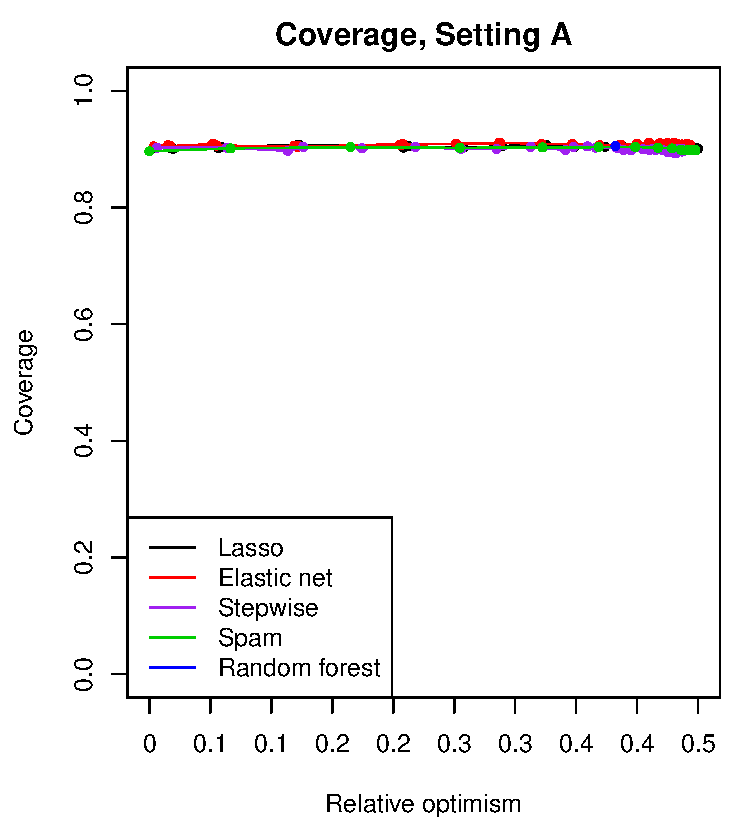
\includegraphics[width=0.32\textwidth]{fig_sim/A_cov.pdf}
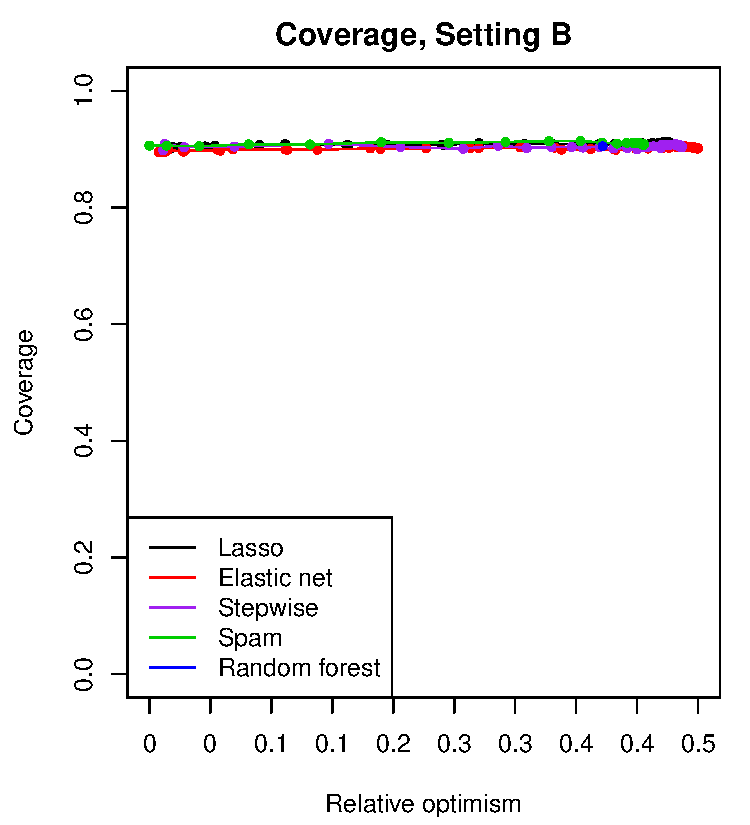
\includegraphics[width=0.32\textwidth]{fig_sim/B_cov.pdf}
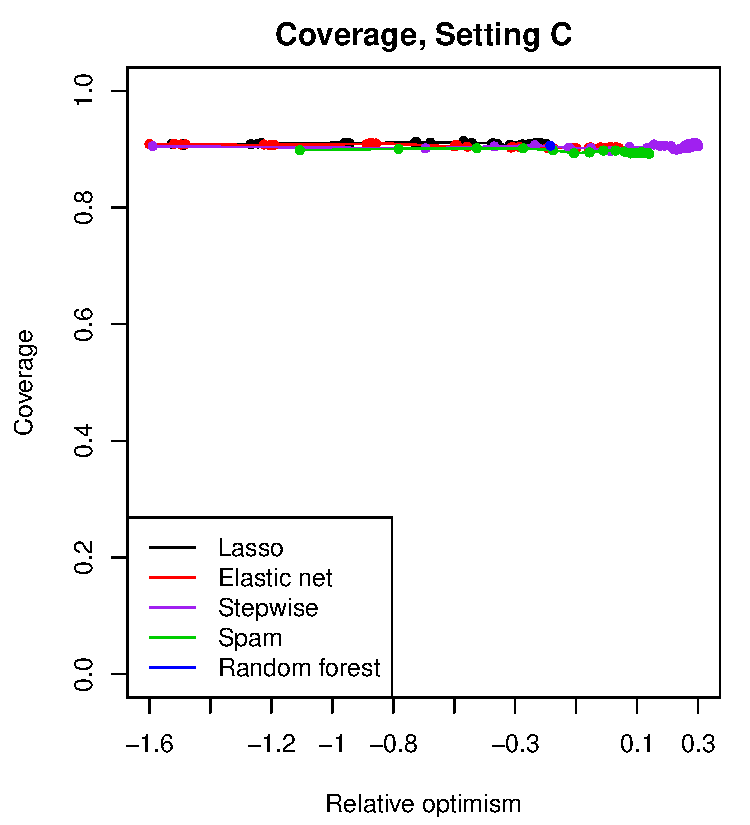
\includegraphics[width=0.32\textwidth]{fig_sim/C_cov.pdf} \\
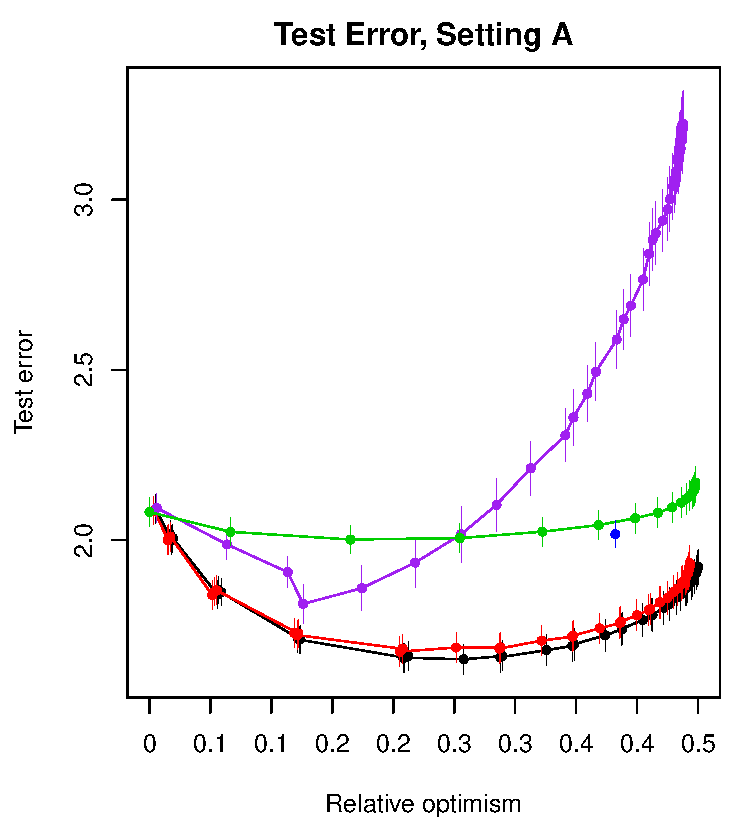
\includegraphics[width=0.32\textwidth]{fig_sim/A_err.pdf}
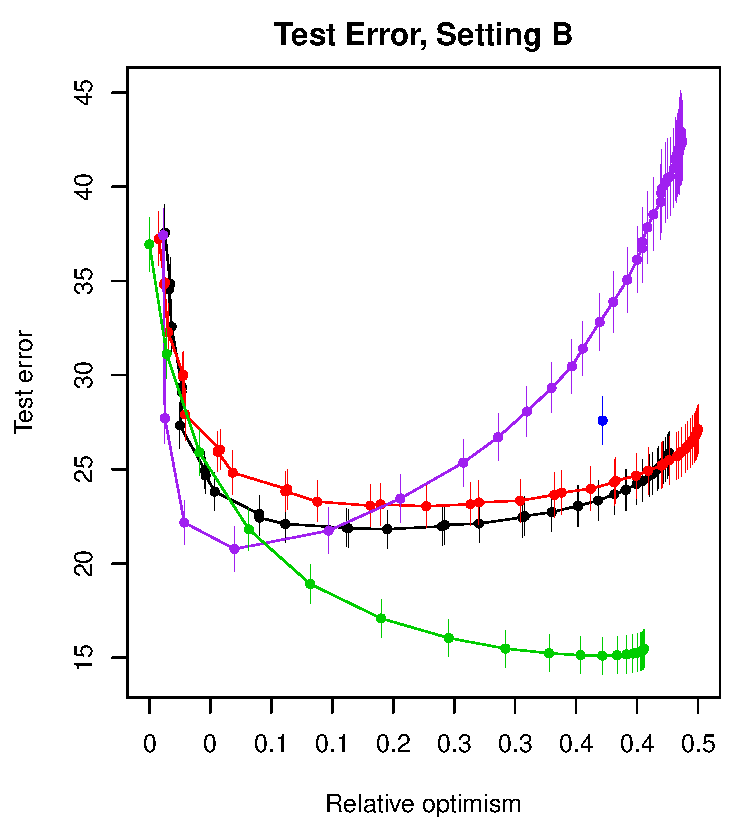
\includegraphics[width=0.32\textwidth]{fig_sim/B_err.pdf}
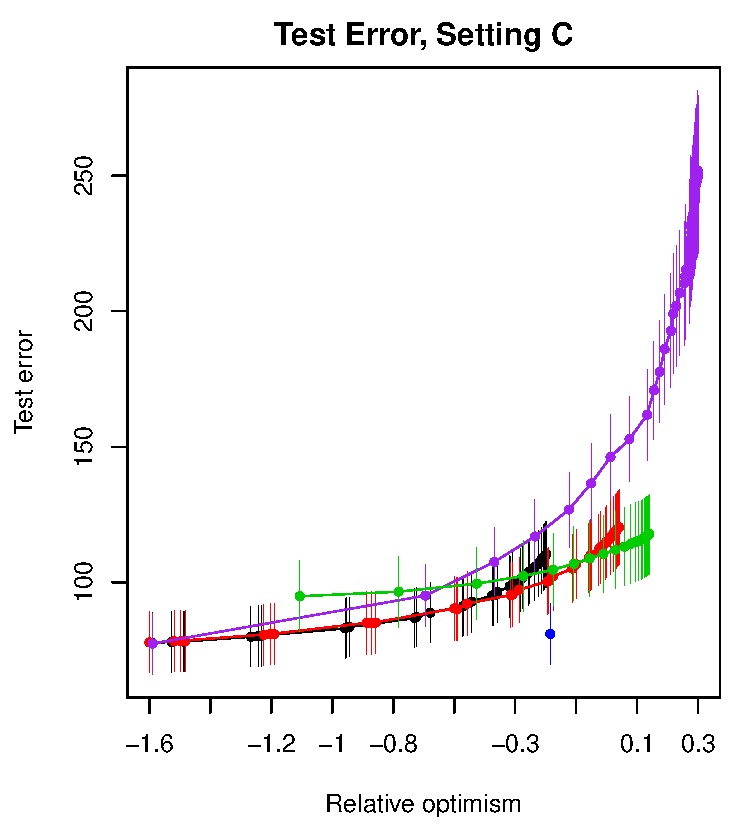
\includegraphics[width=0.32\textwidth]{fig_sim/C_err.pdf} \\
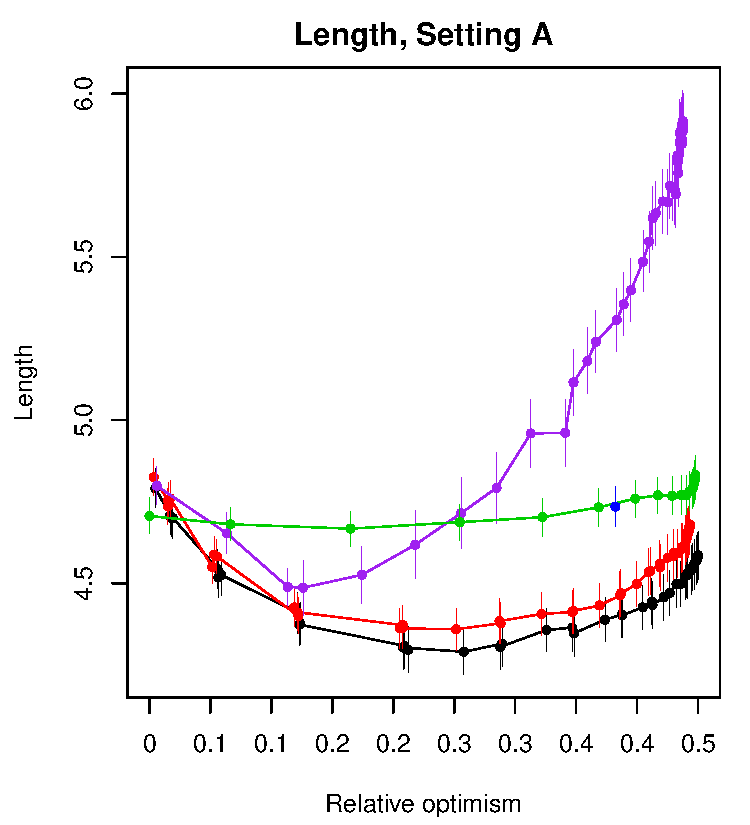
\includegraphics[width=0.32\textwidth]{fig_sim/A_len.pdf}
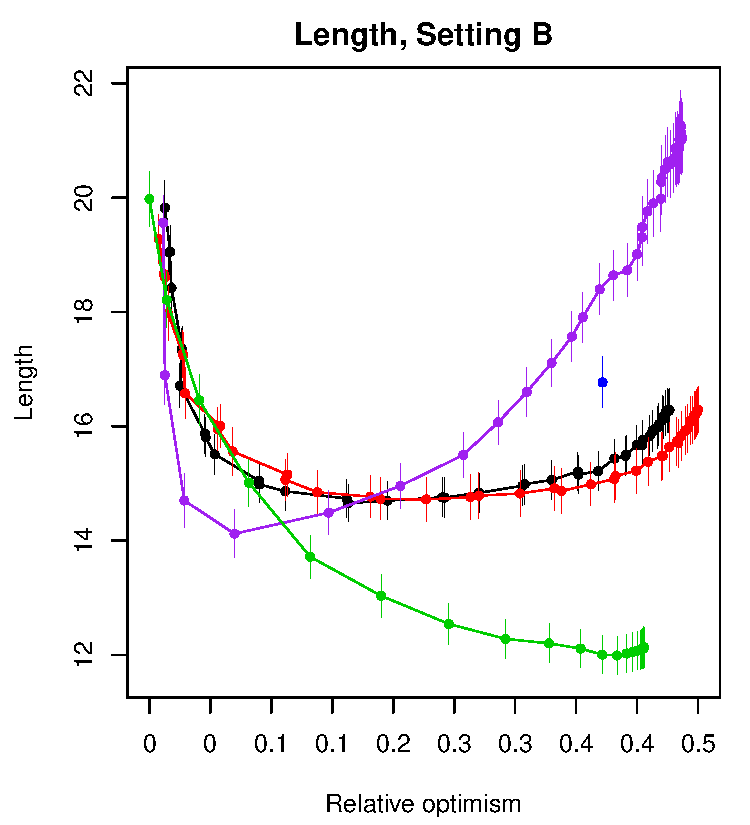
\includegraphics[width=0.32\textwidth]{fig_sim/B_len.pdf}
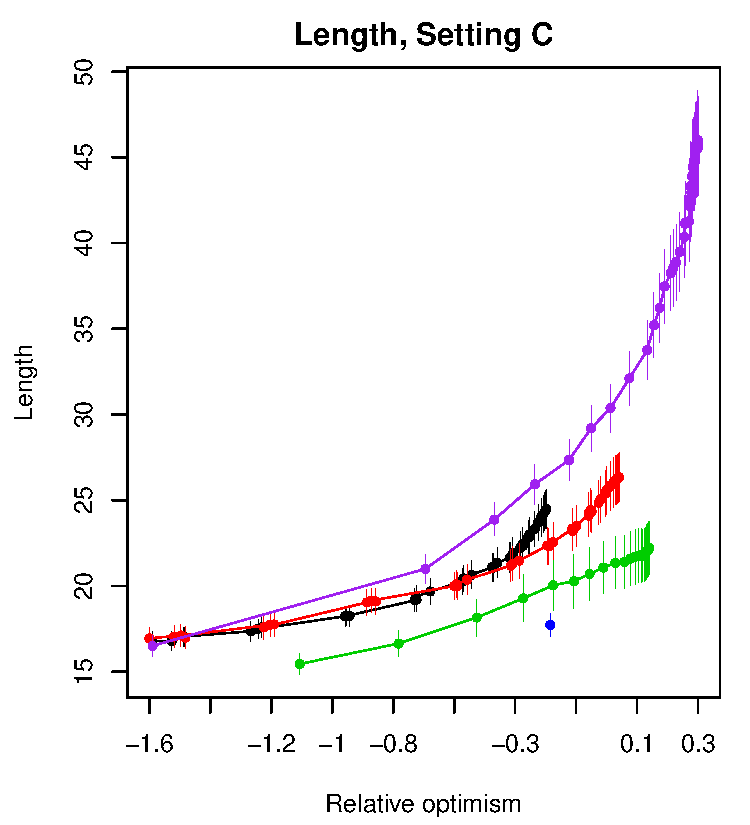
\includegraphics[width=0.32\textwidth]{fig_sim/C_len.pdf} 
\caption{\it Experiments demonstrating the coverage (top row), test error
  (middle row), and average length (bottom row) of split conformal prediction in
  three different simulation settings, and with several different prediction 
  algorithms. The x-axis in each plot sweeps over internal hyperparameters of 
  the algorithms (they are simply put on a common scale using a notion called
  relative optimism). Settings A, B, and C are increasingly challenging, in
  terms of the tractability of prediction. Takeaways: any algorithm, using any 
  hyperparameter value, leads to essentially exactly 90\% coverage in all
  settings (this was the nominal level), as seen in the top row; moreover, test 
  error of the algorithm-hyperparameter pair and average length (or width, these
  are used synonymously) of the prediction set correlate quite strongly. Credit:
  \citet{lei2018distribution}.}       
\label{fig:experiments}
\end{figure}

\subsection{Example}

Now we give an example of split conformal in action, in Figure
\ref{fig:split}. In this simple univariate example (real-valued features), we
split the data randomly and equally into a proper training set (points drawn in
black) and a calibration set (drawn in blue). We use a smoothing spline with 5
degrees of freedom to fit \smash{$\hf_{n_1}$} on the proper training set. The
split conformal prediction band, which is simply computed from an adjusted 
level 90\% quantile of the calibration residuals, and is drawn in orange. 

\begin{figure}
\centering
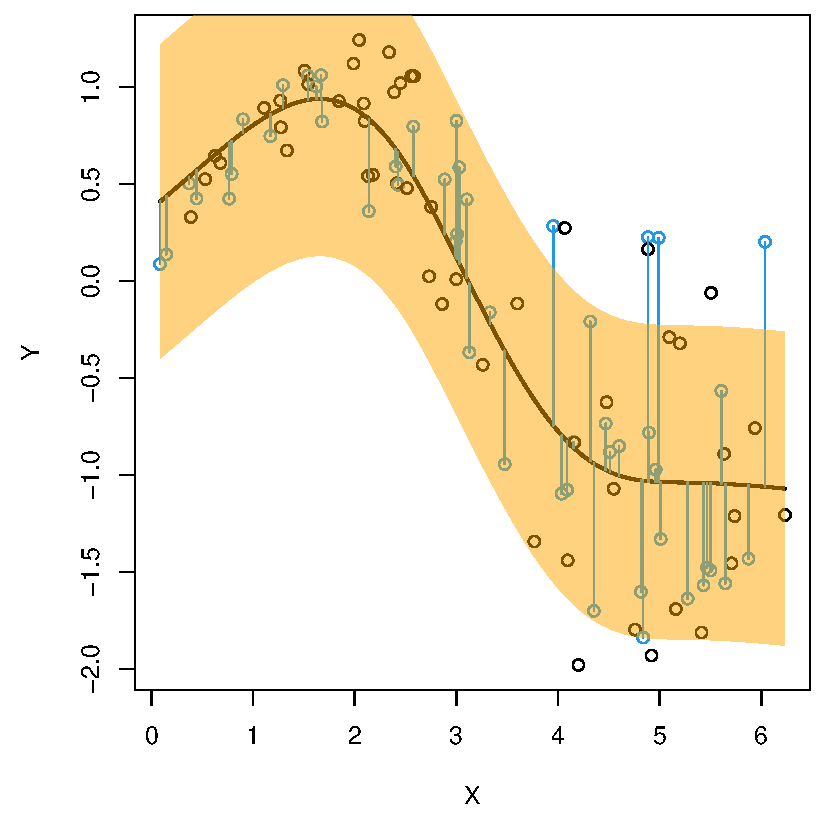
\includegraphics[height=0.33\textheight]{split.pdf}
\caption{\it Example of split conformal prediction, based on a smoothing spline
  with 5 degrees of freedom.} 
\label{fig:split}
\end{figure}

This is guaranteed to have at least 90\% test coverage, when we draw test points
from the same distribution as that used to generate the training data. We can
see that the band is constant-width, by design. This is a function of using the
absolute residual as our conformity score. It is not desirable in the current
example because it will tend to overcover on the left side of the domain, and
undercover on the right side (note that the variance of $Y|X$ is not constant in
this example). We will revisit (and remedy) this later in Section
\ref{sec:local_adaptivity}.   

\subsection{Conditional coverage properties?}

We have seen that split conformal prediction comes with the strong,
distribution-free coverage guarantee in \eqref{eq:coverage_split}. Of course, 
simply by marginalizing over the proper training set, it also has the
unconditional coverage property, 
\[
\P\Big( Y_{n+1} \in \hC_n(X_{n+1}) \Big) \in
\Big[ 1-\alpha, \, 1-\alpha + \frac{1}{n_2+1} \Big).  
\]

Going the other direction, we could ask if it has coverage properties after we
condition on \emph{more} than just the proper training set. If we condition on
both the proper training set and the calibration set, that is, we condition on
the \emph{entire training set}, then when the conformity scores are almost 
surely distinct (or we use a suitably random tie-breaking rule): 
\begin{equation}
\label{eq:coverage_beta_split}
\P\Big(Y_{n+1} \in \hC_n(X_{n+1}) \, \Big| \, (X_i,Y_i), \, i=1,\dots,n \Big) 
\sim \mathrm{Beta}(k_\alpha, n_2+1-k_\alpha), 
\end{equation}
where \smash{$k_\alpha = \lceil (1-\alpha)(n_2+1) \rceil$}. The result in
\eqref{eq:coverage_beta_split} is a consequence of standard facts about order
statistics and you'll prove it on the homework. How do we interpret it? Note,
the only thing random in this probability the test point $(X_{n+1},Y_{n+1})$
(everything else has been conditioned on). Therefore, we can think about it as
follows: \emph{as we draw random calibration sets}, each one being of size $n_2$ 
(containing i.i.d.\ draws from a fixed distribution $P$), the coverage
integrated over a single test point is distributed as $\mathrm{Beta}(k_\alpha,
n_2+1-k_\alpha)$. This distribution has mean   
\[
\frac{k_\alpha}{n_2+1} = \frac{\lceil (1-\alpha)(n_2+1) \rceil}{n_2+1},
\]
exactly as expected. It has variance
\[
\frac{k_\alpha (n_2+1-k_\alpha)}{(n_2+1)^2 (n_2+2)} \approx 
\frac{\alpha (1-\alpha)}{n_2+2}.
\]
Thus when $n_2$ is small, this distribution has considerable variability, and
for any given calibration set in hand, we might see the test coverage looking
far from $1-\alpha$. To give you a more precise sense, Figure \ref{fig:beta} 
plots the density of this beta distribution for $\alpha = 0.1$ and a few values 
of $n_2$.   

\begin{figure}[htb]
\centering
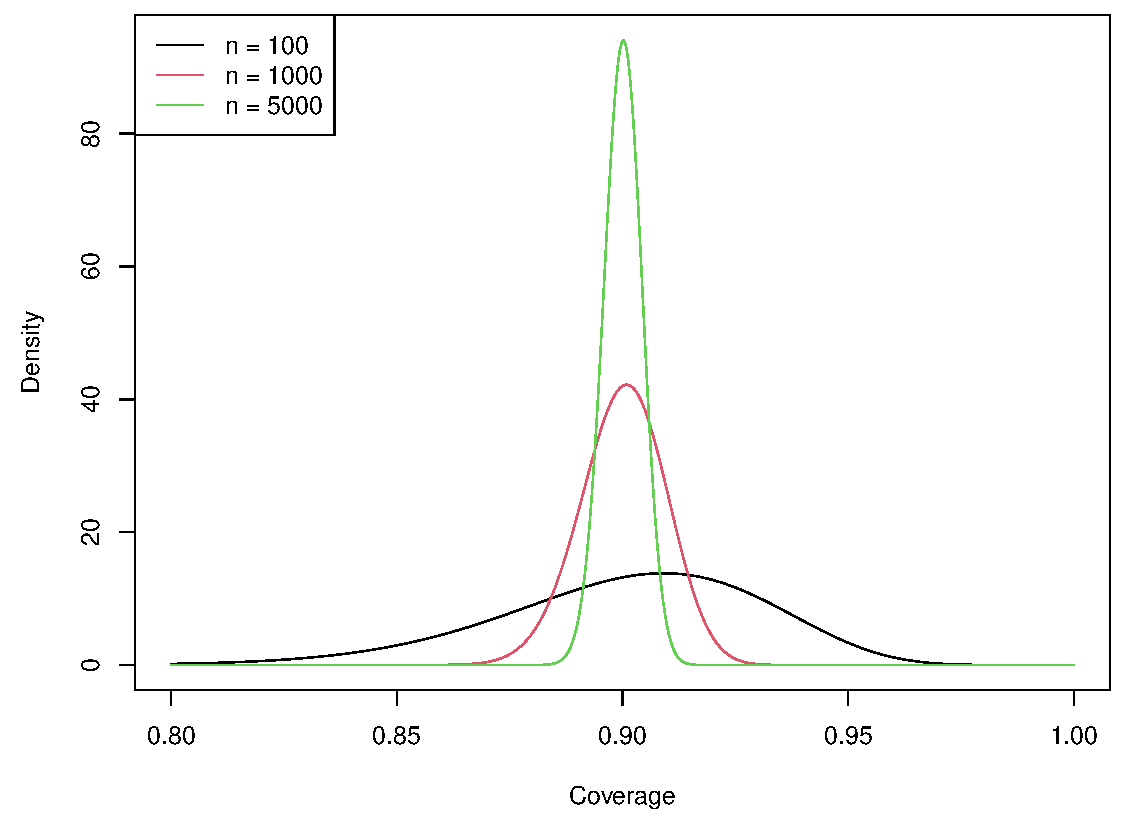
\includegraphics[width=0.75\textwidth]{beta.pdf}
\caption{\it Density of the beta distribution in \eqref{eq:coverage_beta_split}
  that describes the calibration set conditional coverage of split conformal 
  prediction, for $alpha = 0.1$ and a few values of $n_2$.}
\label{fig:beta}
\end{figure}

How about instead conditioning on $X_{n+1}$? This kind of coverage, which we
will call \emph{X-conditional coverage}, would be highly desirable: it would say
that 
\[
\P\Big( Y_{n+1} \in \hC_n(x) \, \Big| \, (X_i,Y_i), \, i \in D_1, \, X_{n+1} = x 
\Big) \geq 1-\alpha, \quad \text{for all $x \in \cX$},
\]
which means that we would cover the response at test feature value $x$. Alas,
this is asking for too much, and in a sense that we will make precise later, in
Section \ref{sec:impossibility}, this is effectively impossible to do without
making assumptions about the distribution $P$ governing the data.

\section{Full conformal prediction}

Is there some way to get guaranteed coverage without splitting the data? Enter 
\emph{full conformal prediction} (often just called conformal prediction). This
method is generally much more expensive and much more complicated than its split
counterpart, but it is nonetheless a beautiful and important idea---and in some
cases, it can indeed be computed efficiently. 

In full conformal prediction, we still abide by the second key idea described
previously, in which we construct residuals in a way that treats all data
symmetrically. We just do it in a more subtle way. Fix any $x \in \cX$, and
suppose that we want to figure out whether any given response value $y \in \R$
should be in our prediction set \smash{$\hC_n(x)$}. We call $y$ in the
\emph{trial} or \emph{query} value.  Now we do something unlike anything we have
seen thus far: we train our prediction algorithm on
\smash{$(X_1,Y_1),\dots,(X_n,Y_n),(x,y)$}---note this is an \emph{augmented}  
training set, with $n+1$ points---to produce a point predictor
\smash{$\hf_{n,(x,y)}$}. We define residuals  
\begin{align*}
R_i^{(x,y)} &= |Y_i-\hf_{n,(x,y)}(X_i)|, \quad i=1,\dots,n, \\
R_{n+1}^{(x,y)} &= |y-\hf_{n,(x,y)}(x)|.
\end{align*}
Then we define a conformal set
\begin{equation}
\label{eq:cset_full}
\hC_n(x) = \Big\{ y : R_{n+1}^{(x,y)} \leq \text{$\lceil (1-\alpha)(n+1) \rceil$
  smallest of $R_1^{(x,y)}, \dots, R_n^{(x,y)}$} \Big\}. 
\end{equation}
The guarantee we get is that 
\begin{equation}
\label{eq:coverage_full}
\P\Big( Y_{n+1} \in \hC_n(X_{n+1}) \Big) \in \Big[ 1-\alpha, \, 1-\alpha +
\frac{1}{n+1} \Big),
\end{equation}
where the lower bound on coverage always holds, and the upper bound holds under
the assumption that the residuals are almost surely distinct once we plug in
for the random test point $(x,y) = (X_{n+1},Y_{n+1})$. Why? After we plug in for
the random test point, and abbreviate
\[
R_i = R_i^{(X_{n+1},Y_{n+1})}, \quad i=1,\dots,n+1,
\]
we can see that \emph{these residuals are all exchangeable}. (To be precise,
this is only true if the algorithm that we use to fit the point predictor
\smash{$\hf_{n,(x,y)}$} is a symmetric function of the training data that it
takes as input, i.e., does not use knowledge of the order in which the training
points were passed.) Therefore
\[
Y_{n+1} \in \hC_n(X_{n+1}) 
\iff \text{$R_{n+1} \leq \lceil (1-\alpha)(n+1) \rceil$ smallest of $R_i$,
  $i=1,\dots,n$}
\]
occurs (by our previous arguments) with probability at least $1-\alpha$, and at
most $1-\alpha+1/(n+1)$ if the residuals are almost surely distinct.

All of the extensions mentioned in the split conformal section, after defining
the basic method based on residual scores, carry over to full conformal. We
summarize these below.

\begin{itemize}
\item Any negatively-oriented and suitably symmetric score function can be used
  in place of the absolute residual score and the guarantee is unchanged. That
  is, define 
  \begin{align*}
  R_i^{(x,y)} &= V\Big( (X_i,Y_i); \, (X_1,Y_1), \dots, (X_n,Y_n), (x,y) \Big)
  \quad i=1,\dots,n, \\ 
  R_{n+1}^{(x,y)} &= V\Big( (x,y); \, (X_1,Y_1), \dots, (X_n,Y_n), (x,y) \Big)
  \end{align*}
  for any function $V$ that is symmetric in its last $n+1$ arguments. This
  function can, for example, train a point predictor on the last $n+1$
  arguments---as long as it treats them symmetrically---and then use it to
  return some score for the first argument. Then the conformal prediction set in
  \eqref{eq:cset_full} still has the same guarantee in \eqref{eq:coverage_full},
  by the same exchangeability arguments. 

\item We can rewrite the conformal set \eqref{eq:cset_full} in equivalent
  quantile and CDF forms:
\begin{align}
\hC_n(x) 
\label{eq:cset_quant_full}
&= \bigg\{ y : R^{(x,y)}_{n+1} \leq \Quantile\bigg( \frac{\lceil (1-\alpha)(n+1) 
  \rceil}{n}; \, \frac{1}{n} \sum_{i=1}^n \delta_{R_i^{(x,y)}} \bigg) \bigg\} \\ 
\label{eq:cset_cdf_full}
&= \bigg\{ y : \frac{1}{n} \sum_{i=1}^n 1\Big\{ R_i^{(x,y)} \leq R^{(x,y)}_{n+1}
  \Big\} \leq \frac{\lceil (1-\alpha)(n+1) \rceil}{n} \bigg\}.   
\end{align}

\item We can always inject auxiliary randomness in order to obtain coverage
  exactly $1-\alpha$ in \eqref{eq:coverage_full}.
\end{itemize}

\subsection{Remarks}

The remarks discussed for split conformal previously also carry over more or
less to full conformal prediction. To summarize briefly: the full conformal band
is protected against overfitting, because now computation of
\smash{$\hf_{n,(x,y)}$} involves the query point $(x,y)$; the band produced by
full conformal under the residual score is often roughly (though not exactly)
constant-width, which is not generally a good property, but can be addressed by
changing the score function (more later); and lastly, in general, the better the
prediction algorithm, the tighter the band will be overall. 

Next we give two further remarks. The first one is on computation: full
conformal is in general \emph{extremely computationally expensive}: for every
$x$ at which we want to compute the prediction set \smash{$\hC_n(x)$} in
\eqref{eq:cset_full}, we need to refit the point predictor 
\smash{$\hf_{n,(x,y)}$} (kernel regression, random forest, neural net, etc.) at 
in principle every $y \in \R$ in order to compute and compare the residuals
\smash{$R_i^{(x,y)}$}, $i=1,\dots,n+1$. This would actually be infinitely
expensive, but in practice of course we would do it over a finite grid of $y$
values, which could still be tremendously expensive. Relatively speaking, split 
conformal is computationally trivial: it is typically dominated by the cost of
fitting the point predictor \smash{$\hf_{n_1}$} once. Due to its extreme
computational cost, full conformal prediction is rarely used in practice, except
for small problem sizes, or with special prediction algorithms that have
something like a ``shortcut'' formula for refitting the point predictor. 
% This includes (but is not limited to) linear and ridge regression, since the  
% Woodbury formula tells us how to efficiently move from a fit on a training set
% of $n$ points to the augmented training set of $n+1$ points with $(x,y)$
% appended.  
Also, it is worth mentioning that in between split and full conformal prediction
are methods that look like cross-validation, and cycle through using different
parts of the data for training and. See \citet{barber2021predictive} for
details.   

The second remark is about interpreting the conformal set via p-values. Observe 
that we can rewrite \eqref{eq:cset_cdf_full} once more as
\[
\hC_n(x) = \bigg\{ y : \underbrace{\frac{1}{n} \sum_{i=1}^n 1\Big\{ R_i^{(x,y)} 
  > R^{(x,y)}_{n+1} \Big\}}_{p(y)} \geq \frac{\lfloor \alpha (n+1) \rfloor}{n} 
\bigg\}.  
\]
Informally, we can interpret the fraction of residuals larger than the test
residual, which we denote by $p(y)$, as a p-value for the null hypothesis $H_0: 
Y_{n+1} = y$. Thus we can think of conformal prediction as using $y$ as a
pivotal value, and \emph{keeping all of values $y$ for which we do not reject}
the null hypothesis, which it does by comparing $p(y)$ to an adjusted
significance level of \smash{$\lfloor \alpha (n+1) \rfloor / n$}.

\subsection{Example}

Figure \ref{fig:full} gives an example of full conformal in action. The
underlying data is the same as in Figure \ref{fig:split}, but for the prediction
algorithm we now use a smoothing spline with 15 degrees of freedom (this allows
the influence of the query point $(x,y)$ on the spline fit to be more
visible). We demonstrate how to calculate the prediction set at a single value
$x=4.75$, marked in blue. We iterate through a grid of query response values,
and for each such value $y$, we compute the smoothing spline fit using $n+1$
points: the original data set and $(x,y)$. We then record the fraction $p(y)$ of
residuals larger than the test residual. Figure \ref{fig:full} visualizes the
results for 5 such grid values, and then in the bottom right panel, displays the
90\% prediction set, defined by all $y$ for which \smash{$p(y) \geq \lfloor
  \alpha (n+1) \rfloor / n \approx 0.1$} (we can think of this as thresholding
the p-value histogram drawn along the right axis).

\begin{figure}[p]
\centering
\hspace{-10pt}
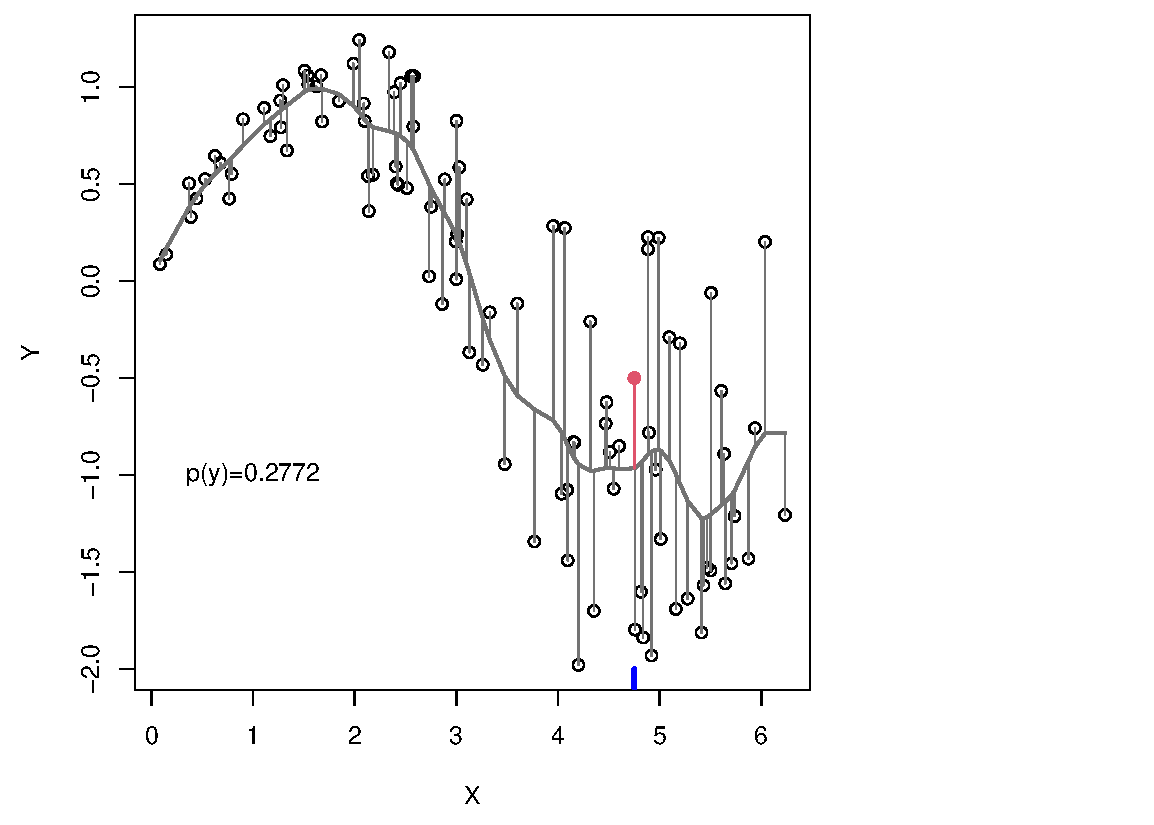
\includegraphics[width=0.55\textwidth]{fig_full/5.pdf} 
\hspace{-50pt}
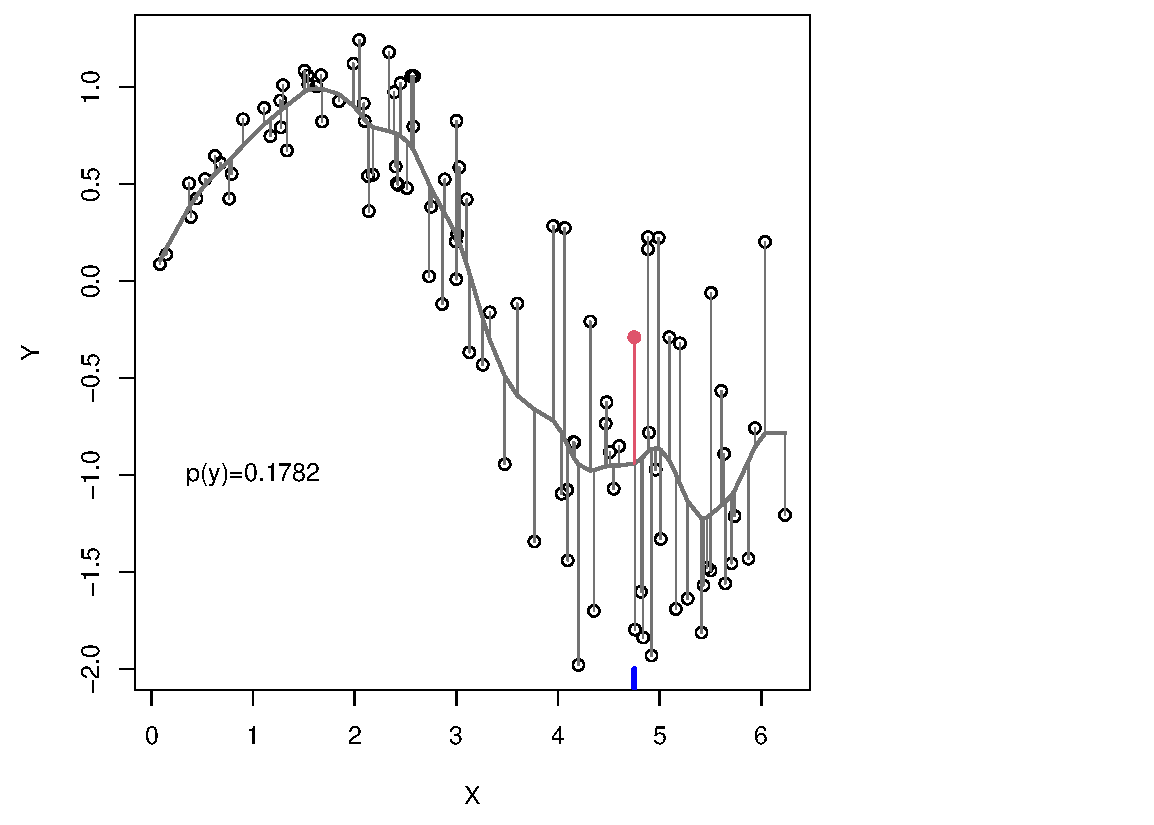
\includegraphics[width=0.55\textwidth]{fig_full/9.pdf} \\
\hspace{-10pt}
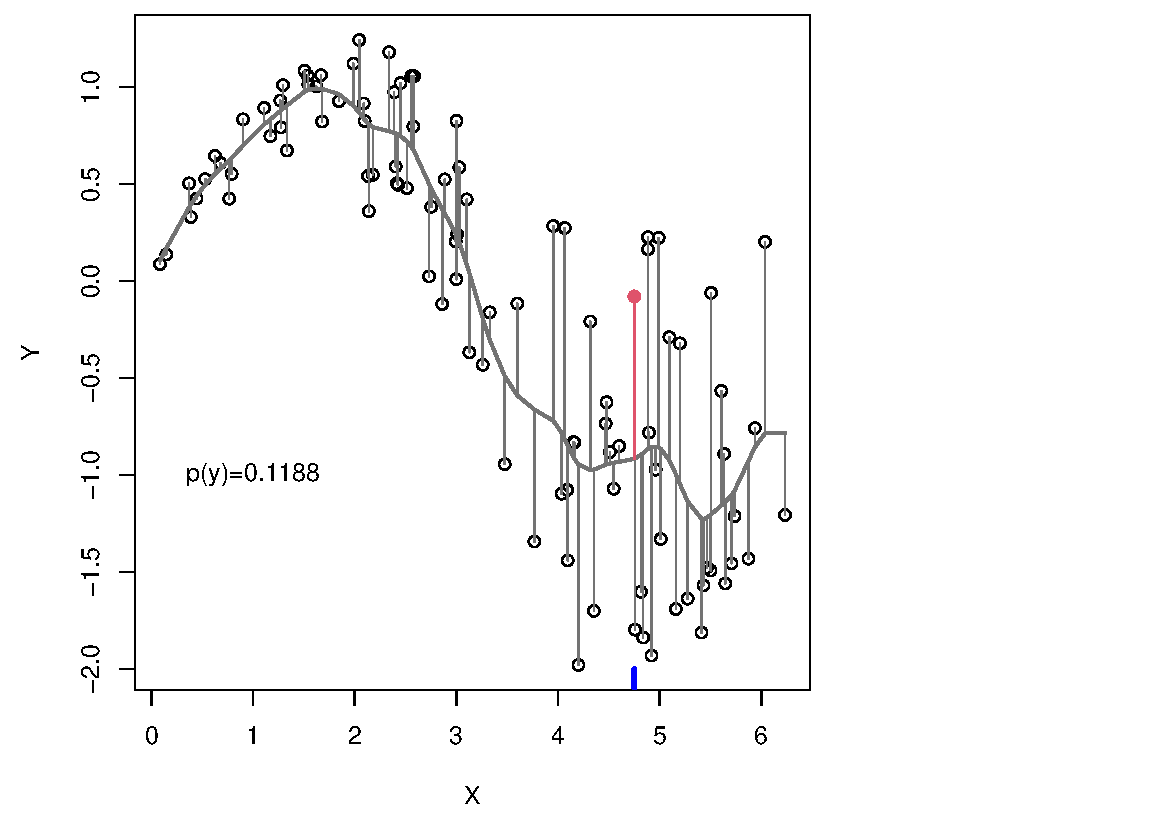
\includegraphics[width=0.55\textwidth]{fig_full/13.pdf} 
\hspace{-50pt}
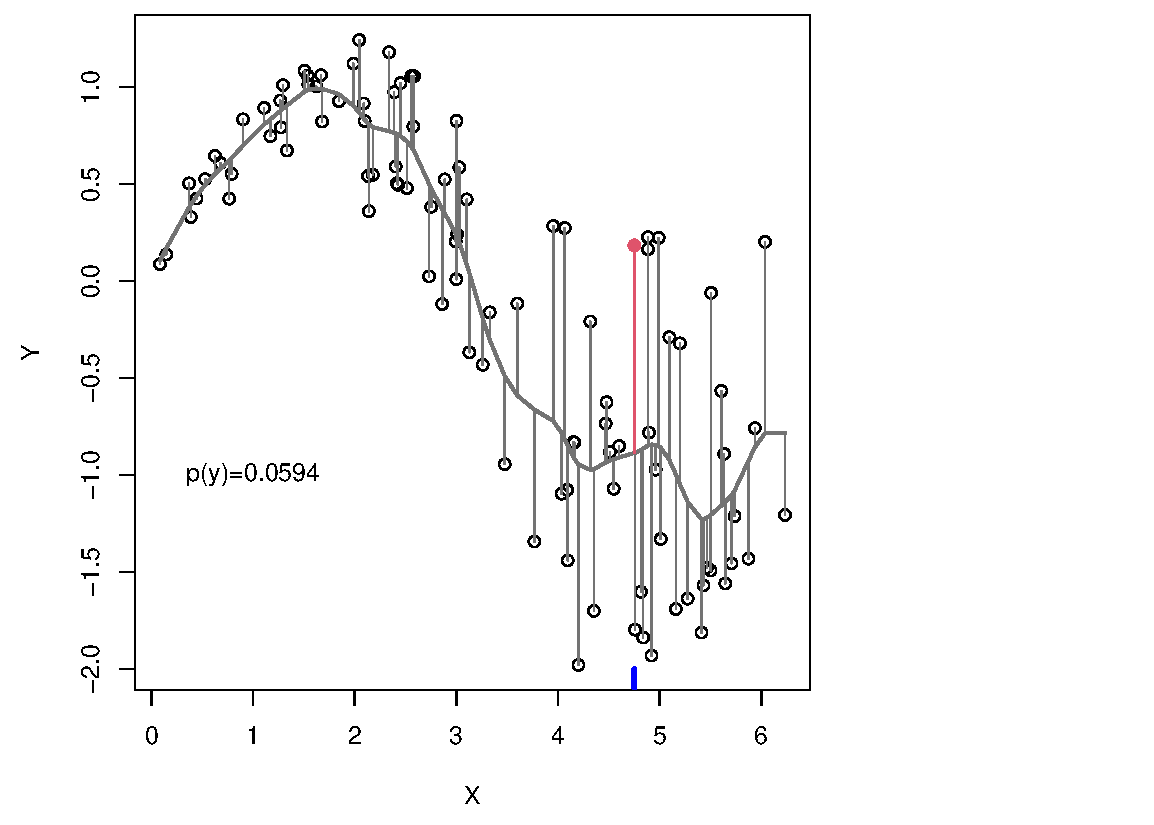
\includegraphics[width=0.55\textwidth]{fig_full/18.pdf} \\
\hspace{-10pt}
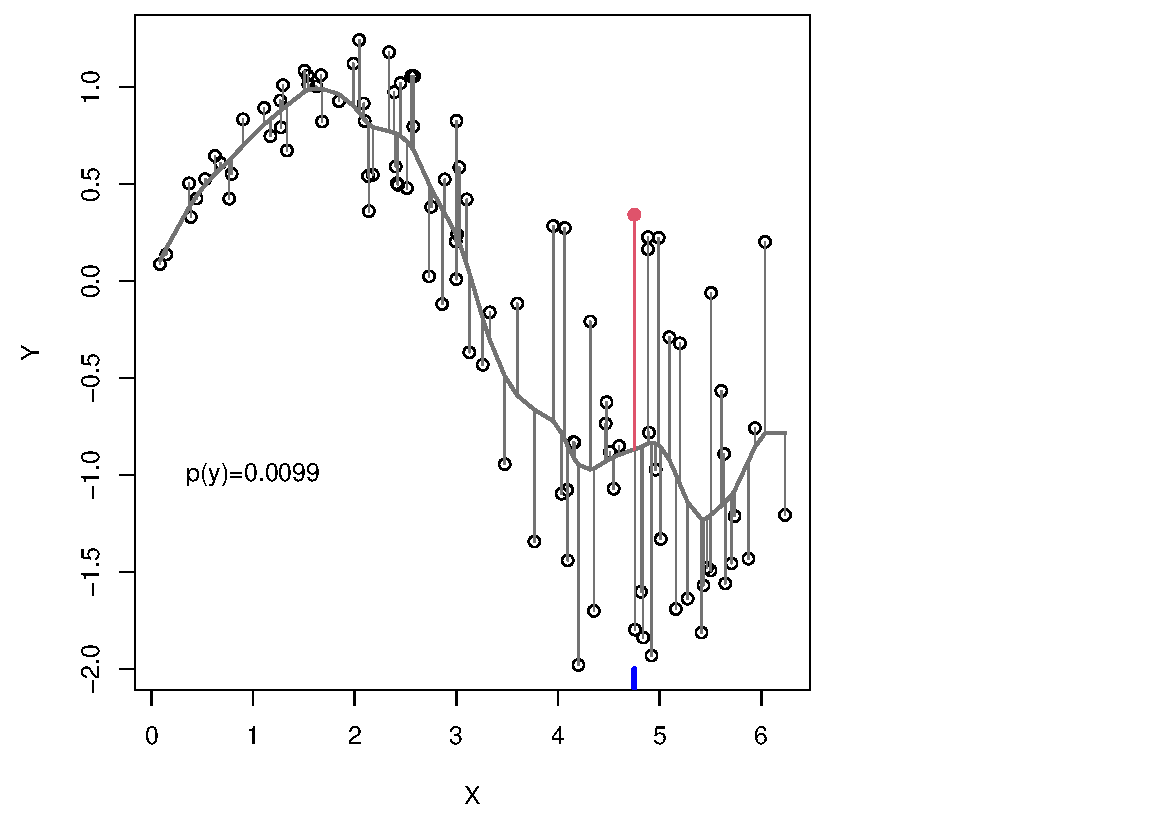
\includegraphics[width=0.55\textwidth]{fig_full/21.pdf} 
\hspace{-50pt}
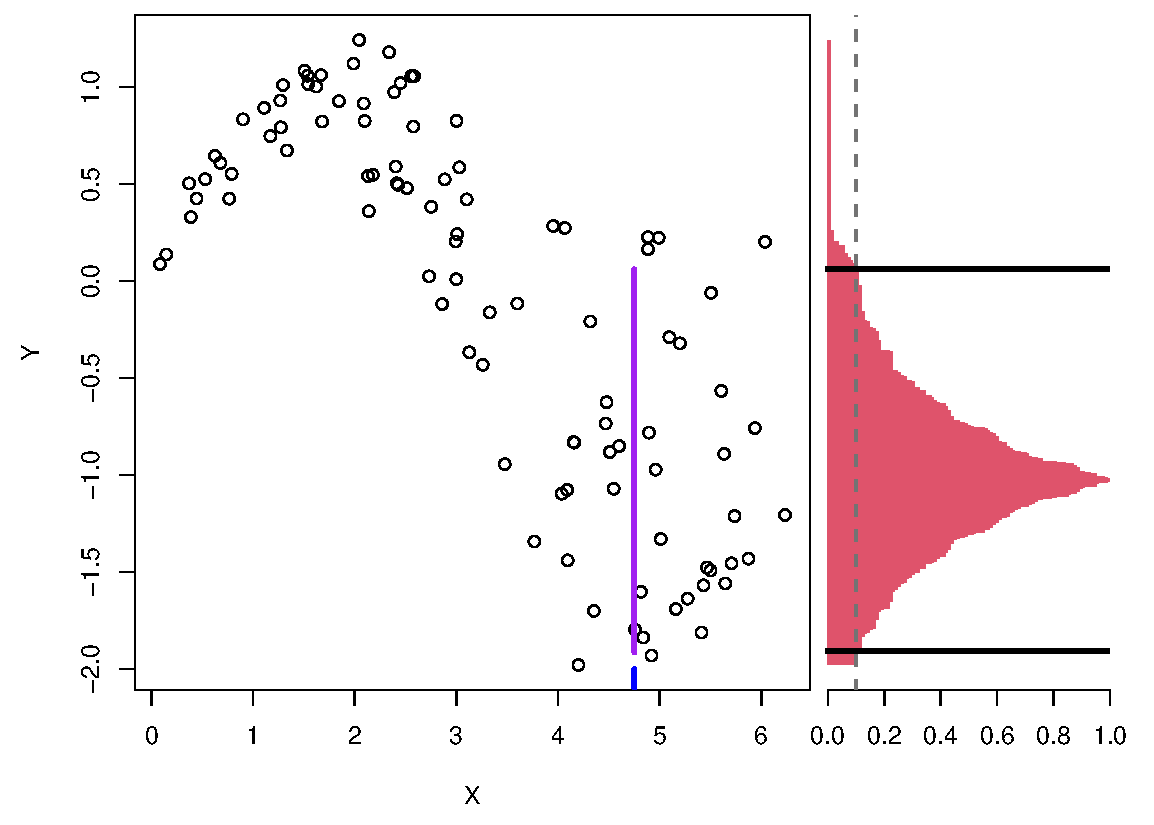
\includegraphics[width=0.55\textwidth]{fig_full/28.pdf} 
%\animategraphics[autoplay,loop,poster=last,height=0.33\textheight]{3}{fig_full/}{1}{28}
\caption{\it Example of full conformal prediction, where the prediction
  algorithm is a smoothing spline with 15 degrees of freedom.}
\label{fig:full}
\end{figure}

\subsection{Impossibility of X-conditional coverage}
\label{sec:impossibility}

Returning to the issue of X-conditional coverage raised previously, here we drop
some disappointing news: conformal prediction methods do not achieve this in
general. The story is actually more grim: no method does, in a meaningful
way, in the distribution-free setting. If \smash{$\hC_n$} is any prediction band
such that  
\[
\P\Big( Y_{n+1} \in \hC_n(x) \, \Big| \, X_{n+1} = x \Big) \geq 1-\alpha, \quad 
\text{for any $P$, and $P_X$-almost every $x$},
\]
then \citet{lei2014distribution, vovk2012conditional} show that (paraphrasing
their results, as done in Proposition 2.2 of \citet{barber2021limits}):
\[
\E \Big[ \mu(\hC_n(x)) \Big] = \infty, \quad \text{for any $P$, and
  $P_X$-almost every non-atom point $x_0$}. 
\]
As before, $\mu$ denotes Lebesgue measure and $P_X$ is the feature distribution
associated with $P$. A non-atom point $x_0$ of $P_X$ is one for which
$P_X(B_\delta(x_0)) \to 0$ as $\delta \to 0$, where $B_\delta(x_0)$ is the
$\ell_2$ ball of radius $\delta$ centered at $x_0$. Thus, in effect, the above
says that any prediction band which claims to cover at almost every $x$, for
every joint distribution $P$, must be infinite in size at any point $x_0$ at
which we do not have a positive probability of seeing duplicate observations. 
You'll explore more of the details on your homework.  

\section{Improving local adaptivity}
\label{sec:local_adaptivity}

Even though X-conditional coverage is effectively impossible in the
distribution-free setting, in the sense made precise previously, this \emph{does
  not} mean that different methods cannot have widely different behaviors in
practice, when it comes to their ability to deliver approximate X-conditional
coverage. We will broaden our terminology and perspective and use \emph{local
  adaptivity} of a prediction band as a term that refers to its ability to
shrink the band at values of $x$ at which prediction is easy, and inflate it at
values of $x$ at which prediction is hard. This is admittedly somewhat vague,
but because X-conditional coverage isn't really our precise goal, local
adaptivity is a better notion to keep in mind.

There are different methods for obtaining better local adaptivity. The ones
covered in this lecture all have to do with simply changing the conformity
score. Below we cover two options in regression. 

\subsection{Studentized residuals}

A simple variant on the residual score is what we call a \emph{studentized
  residual}. We describe the idea for split conformal prediction (the full
conformal extension is similar). On $D_1$, we fit both a point predictor
\smash{$\hf_{n_1}$} and a ``spread predictor'' \smash{$\hat\sigma_{n_1}$}, which 
is designed to predict (say) the standard deviation of \smash{$|Y -
  \hf_{n_1}(X)|$} at $X = x$. Then on $D_2$, we compute ``studentized'' or 
normalized residuals 
\[
R_i = \frac{|Y_i - \hf_{n_1}(X_i)|}{\hat\sigma_{n_1}(X_i)}, \quad i \in D_2, 
\]
and as before \smash{$\hq_{n_2} = \lceil (1-\alpha)(n_2+1) \rceil$ smallest of
  $R_i$, $i \in D_2$}. The conformal set is now   
\begin{equation}
\label{eq:cset_std_split}
\hC_n(x) = \Big[ \hf_{n_1}(x) - \hat\sigma_{n_1}(x) \hq_{n_2}, \, 
\hf_{n_1}(x) + \hat\sigma_{n_1}(x) \hq_{n_2} \Big],   
\end{equation}
whose width we can see adapts according to \smash{$\hat\sigma_{n_1}$}. The
guarantee is just as before, in \eqref{eq:coverage_split}. Figure
\ref{fig:student} gives an example.  

\begin{figure}[htb]
\centering
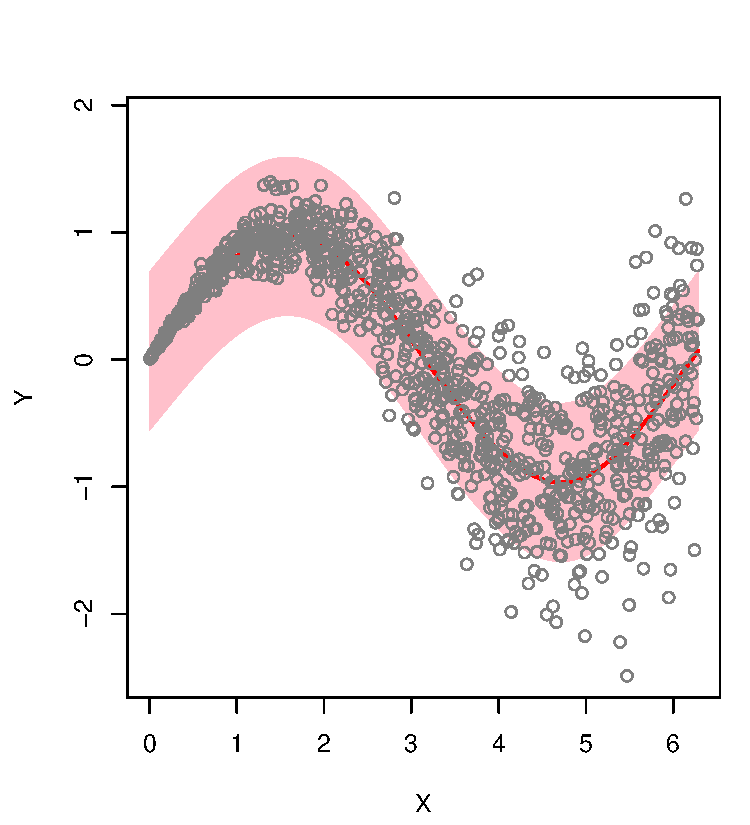
\includegraphics[width=0.49\textwidth]{split_usual.pdf}
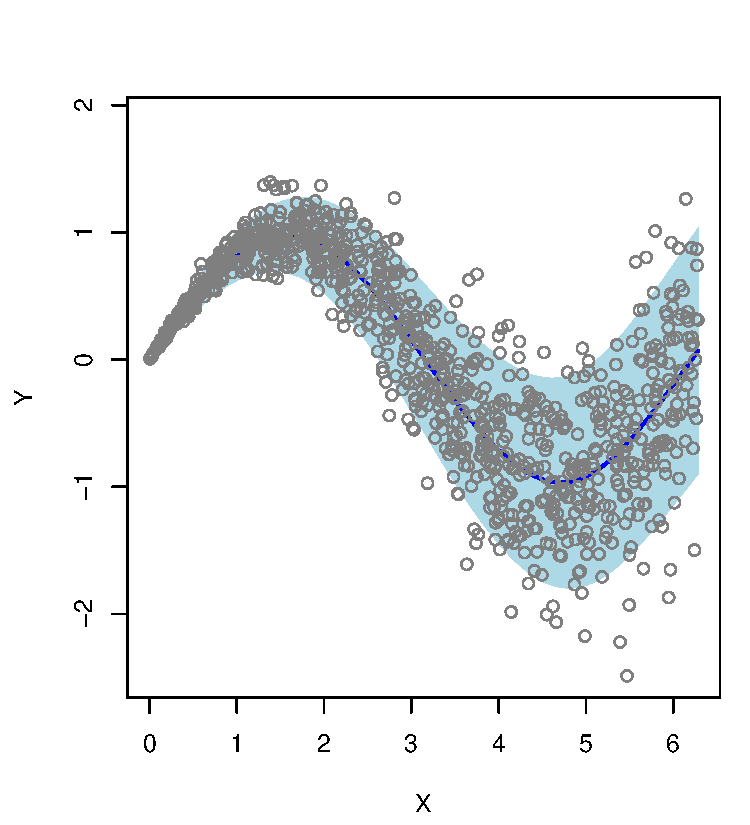
\includegraphics[width=0.49\textwidth]{split_student.pdf}
\caption{\it Examples of split conformal prediction with the usual residual
  score (left panel) and the studentized residual score (right panel). The data
  comes from the same generative model as in Figures \ref{fig:split} and 
  \ref{fig:full}. We can see that the studentized residual adapts to the local
  hardness of prediction (and delivers something closer to conditional
  coverage). Credit: \citet{lei2018distribution}.} 
\label{fig:student}
\end{figure}

\subsection{Quantile regression}

There are two issues that can make studentized residuals fall short in practice.   

\begin{enumerate}
\item If \smash{$\hf_{n_1}$} is complex, then little information is left on the
  proper training set in order to fit \smash{$\hat\sigma_{n_1}$} (because the
  proper training residuals will be close to zero). This can be addressed with
  further data splitting, but that comes at a cost of statistical efficiency. 

\item More broadly, it does not need to be true that the variance of $Y|X=x$ and
  the level $1-\alpha$ quantile of this distribution are always tied together;
  in some problem settings they can even have opposing behaviors. Note that the
  former is being targeted by studentized residuals, but the latter is what
  should really be targeting in prediction bands.       
\end{enumerate}

\citet{romano2019conformalized} show that both of these can be addressed by
changing our perspective on the point predictor itself: why not have it predict
the level $1-\alpha$ quantile of the response at $X=x$ directly? (As opposed to
predicting the mean of the response at $X=x$, which is what generic regression
methods do.) 

Their proposal, called \emph{conformalized quantile regression} (CQR), works as
follows, in the split setting (the full version is similar). We first fit two
point predictors, denoted \smash{$\hf^{\alpha/2}_{n_1}$} and
\smash{$\hf^{1-\alpha/2}_{n_1}$}, on the proper training data $(X_i,Y_i)$, $i  
\in D_1$. Here each \smash{$\hf^\tau_{n_1}(x)$} is estimates the level $\tau$
quantile of $Y|X=x$. This can be obtained from a variety of quantile regression  
methods, which often only require a change of the loss function from a generic
regression method. Then we form calibration set scores    
\[
R_i = \max\Big\{\hf^{\alpha/2}_{n_1}(X_i) - Y_i, \, 
Y_i - \hf^{1-\alpha/2}_{n_1}(X_i) \Big\}, \quad i \in D_2, 
\]
and as before \smash{$\hq_{n_2} = \lceil (1-\alpha)(n+1) \rceil$ smallest of
  $R_i$, $i \in D_2$}. The CQR set is now  
\begin{equation}
\label{eq:cset_cqr_split}
\hC_n(x) = \Big[ \hf^{\alpha/2}_{n_1}(x) - \hq_{n_2}, \,
\hf^{1-\alpha/2}_{n_1}(x) + \hq_{n_2} \Big].
\end{equation}
which enjoys the same guarantee as in \eqref{eq:coverage_split}. 

In the example from Figure \ref{fig:student}, the data set is large enough and
the point predictor stable enough that CQR (not shown) provides little gain over
studentized residuals. However, in other examples, it can provide a clear  
gain. See \citet{romano2019conformalized}. Still, studentized residuals (or
variants thereof) remain in fairly common use since we can use
``out-of-the-box'' regression methods to fit each of \smash{$\hf_{n_1}, 
  \hat\sigma_{n_1}$} in sequence.

\section{Conformal classification}

In this last section, we briefly cover conformal prediction for classification
problems. The story is much the same, but we need different conformity score
functions, since residual or quantile regression scores are not generally
appropriate in classification. Below we cover a standard choice, based on
predicted probabilities. Then we cover a choice that is designed to have better
local adaptivity, based on cumulative probabilities. Throughout, we take $\cY = 
\{1,\dots,K\}$.      

\subsection{Likelihood scores}

We describe the idea for split conformal formulation (full conformal being
similar). We first fit a probabilistic classifier \smash{$\hf_{n_1}$} to the
proper training  data $(X_i,Y_i)$, $i \in D_1$. That is, to be clear, 
\[
\text{$\hf_{n_1}(x; k)$ estimates $\P(Y=k \,|\, X=x)$, for each
  $k=1,\ldots,K$}. 
\]
We then form calibration set scores,
\[
R_i = \hf_{n_1}(X_i; Y_i), \quad \in D_2.
\]
In words, each $R_i$ is the probability or likelihood assigned to the correct
class (on the unseen observation $(X_i,Y_i)$ from the calibration set). Thus
note that this is a positively-oriented score. We let
\[
\text{$\hq_{n_2} = \lfloor \alpha (n_2+1) \rfloor$ smallest of $R_i$, $i \in
  D_2$},  
\]
and define the conformal set
\[
\hC_n(x) = \Big\{ k : \hf_{n_1}(x; k) \geq \hq_{n_2} \Big\}.
\]
This has precisely the same guarantee as in \eqref{eq:coverage_split}.

\subsection{Cumulative likelihood}

\begin{figure}[tb]
\centering
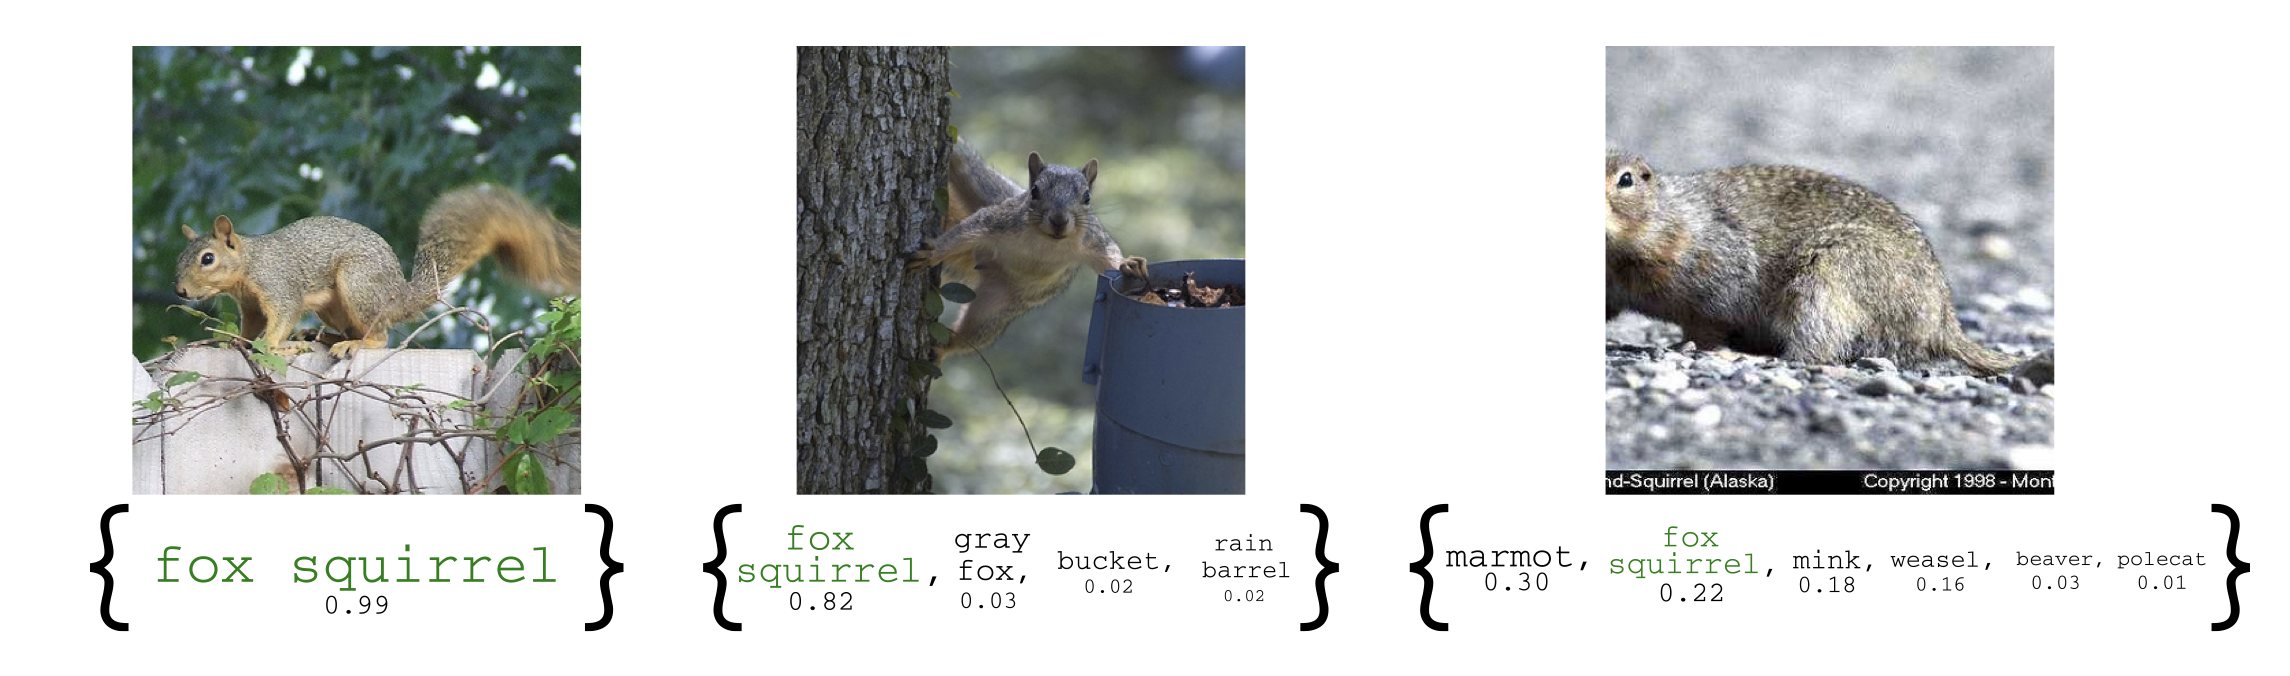
\includegraphics[width=\textwidth]{raps.png}
\caption{\it Examples of RAPS, which is conformal prediction with a regularized
  version of the cumulative likelihood score. The true label in each case is
  ``fox squirrel'', and we can see that the prediction sets adapt appropriately
  in size to the hardness of the classification task. Credit:
  \citet{angelopoulos2021uncertainty}.} 
\label{fig:raps}
\end{figure}

To make the conformal prediction sets more adaptive (still in the context of
having fit a probabilistic classifier \smash{$\hf_{n_1}$} on $D_1$),
\citet{romano2020classification} propose a conformity score based on cumulative
likelihood, defined as follows. For each $i \in D_2$, let $\pi_i$ be the
permutation of $1,\ldots,K$ that sorts the predicted probabilities
\smash{$\hf_{n_1}(X_i; k)$}, $k=1,\dots,K$ in decreasing order, so that  
\[
\hf_{n_1}(X_i; \pi_i(1)) \geq \hf_{n_1}(X_i; \pi_i(2)) \geq \cdots \geq 
\hf_{n_1}(X_i; \pi_i(K)). 
\]
The the conformity scores are 
\[
R_i = \sum_{j=1}^{k_i} \hf_{n_1}(X_i; \pi_i(j)), \quad \text{where $\pi_i(k_i) =
  Y_i$, for each $i \in D_2$}.
\]
In words, each $R_i$ is the cumulative probability of all classes considered
``at least as likely'' as the true one, by our probabilistic classifier. Note
that this is negatively-oriented (if the true class is assigned a very low
probability, then the cumulative probability of all classes ``at least as
likely'' as it will be very high). Hence we let
\[
\text{$\hq_{n_2} = \lceil (1-\alpha)(n_2+1) \rceil$ smallest of $R_i$, $i \in 
  D_2$},  
\]
and define the conformal set
\[
\hC_n(x) = \{ \pi_x(1), \ldots, \pi_x(k_x) \}, \quad \text{where} \; 
k_x =  \min\Bigg\{ k : \sum_{j=1}^k \hf_{n_1}(x; \pi_x(j)) \leq \hq_{n_2} 
\Bigg\}.
\]
This has precisely the same guarantee as in \eqref{eq:coverage_split}.

\citet{angelopoulos2021uncertainty} refer to this method as \emph{adaptive
  prediction sets} (APS) and define a regularized version called RAPS that often
delivers much smaller sets in practice. Figure \ref{fig:raps} gives a few
examples of RAPS from their paper.

\bibliographystyle{plainnat}
\bibliography{../../common/ryantibs}

\end{document}
